\chapter{Úvod}
Vývoj centrálního zásobování teplem prošel od dob svého vzniku několika fázemi.
Z hlediska dnešní doby je nejvýznamnější výměna starých parovodů za
prefabrikované horkovody, čímž dochází ke snížení přestupu tepla z rozvodů do
jejich okolí a snížení nákladů při stavbě nových částí sítě. Z hlediska
několika budoucích dekád je žádoucí transformace na obnovitelné, plně
udržitelné a efektivní zásobování teplem. To přináší nové technologické výzvy
související zejména s integrací obnovitelných zdrojů, využitím odpadního tepla
a celkově snižováním emisí oxidu uhličitého. Je totiž obecně přijímaným faktem,
že pro smysluplnou implementaci obnovitelných zdrojů tepla a odpadní, jež lze
obecně považovat za nízkoteplotní zdroje, je nutné dále snižovat
teplotu v teplárenských rozvodech. Snižovaní této teploty má za následek další
redukci ztrát při distribuci tepla, ale komplikuje efektivní předávání tepla na
straně spotřebitelů a zvyšuje provozní náklady čerpadel. Proto je nutné do sítě
implementovat další prvky, jež umožní efektivní zvýšení teploty blízko
samotných spotřebitelů. Jako další problém lze zmínit značnou nestálost
obnovitelných zdrojů tepla. Se zvyšující se komlexností sítí bude nutné zlepšit
možnosti optimalizace jejich provozu. Toho lze dosáhnout například prediktivním
řízením využívající matematické modely a vhodnou koncepcí akumulace tepla
společně s předpovědí počasí a predikcí množství potřebného tepla. Systémy, jež
se budou schopny vypořádat s těmito a dalšími výzvami lze obecně nazvat čtvrtou
generací teplárenských sítí \cite{Lund2014}.

Množství hmoty, které ovlivňuje fyzikální dynamiku rozsáhlých energetických
systémů již samo o sobě naznačuje komplexnost potenciálního matematického
modelu (digitálního dvojčete či prototypu). Užitečnost takových modelů roste
společně s jejich výpočtovou rychlostí a také s rychlostí s jakou je možné tyto
modely sestavovat. Deklarativní programování může výrazně zjednodušit proces
kompletace z jednotlivých komponent. V numerickém řešení pak modely obvykle
využívají matice, jež se v nich objevují zpravidla kvůli tzv. linearizaci
diferenciálních rovnic (tedy rovnic řídících fyzikální chování). Výpočtová
rychlost je pak úměrná velikosti a hustotě těchto matic. V dnešní době se
můžeme často setkat se snahou o zmenšování matic pomocí redukce směrem k tzv.
jedno‑dimenzionálním modelům. Další výrazný vliv na výpočetní rychlost má
programovací jazyk použitý pro implementaci (strojový kód zpravidla poběží
rychleji než kód interpretovaný) a také míra a provedení paralelizace
algoritmů.

Počítačové učení je moderní vědecká disciplína, která umožňuje vytvářet modely
pomocí dat a to na základě optimalizace parametrizovaných programů. V této
oblasti existuje celá řada numerických struktur umožňující až univerzální
aproximaci (např. neuronové sítě).

Cílem této disertační práce je vytvoření nástrojů (softwarových balíčků) pro
modelování komponent tepelného zásobování s ohledem na optimalizaci numerické
efektivnosti simulací s využitím deklarativního programování a počítačového
učení. Model tepelného zásobování zde poslouží jako studijní příklad jejich
aplikace.

\chapter{Současné shrnutí stavu poznání}
\label{struktura}
V této kapitole jsou uvedeny relevantní rovnice pro modelování CZT. Dále je
provedena stručná rešerše literatury na kterou tato práce navazuje, nebo
využívá její poznatky. Následně jsou popsány použitelné výpočetní přístupy
a metody spolu s aspekty, ovlivňující numerickou efektivnost simulací.

\section{Stručná historie rozvoje teplárenství}
\label{sec:history}
Teplárenské potrubí slouží k dopravě tepla od jeho výrobce k jeho spotřebiteli
pomocí teplonosného média. V minulosti se jako první teplonosné médium
používala pára o teplotě i přes 240 °C. Tyto rozvody generovaly značné tepelné
ztráty a kvůli vysokému tlaku (naakumulované tlakové energii) i vážné
explozivní nehody. Kvůli kondenzaci páry ve vratném potrubí docházelo k jeho
korozi. Pára se jako hlavní teplonosné médium stále využívá například v Paříži
či Manhattanu. Nástupce tohoto provedení využíval tlakovou horkou vodu o
teplotě přes 100 °C. Kvůli nestlačitelnosti vody se výrazně omezily explozivní
nehody.
Motivací bylo snížení tepelných ztrát a možnost lepší implementace kombinované
výroby tepla a elektrické energie v městských oblastech. Poté přišel trend
snižování teploty v rozvodech pod 100 °C. Stále byla využívána tlaková horká
voda. Začalo se značně využívat prefabrikované a před-izolované potrubí
snižující množství lidské práce při výstavbě a obnově rozvodů. Začala se
využívat lokální paliva, odpady a na několika místech i sluneční či geotermální
energie.

V následujících dvou až třech dekádách bude trend snižování teploty v
rozvodech pokračovat ruku v ruce se snižující se náročností budov na prostorové
vytápění. Bude existovat snaha o výraznější implementaci obnovitelných a
odpadních zdrojů energie a k využívání synergií. Pro snížení následků fluktuací
zdrojů, budou využívány akumulační systémy a matematické modely jednotlivých
součástí systému se zaměřením na jejich dynamiku jakožto základ prediktivního
řízení využívající předpovědi meteorologických podmínek \cite{Lund2014}.

\section{Tepelná dynamika teplárenských rozvodů/potrubí}
\label{sec:HeatDynamics}
Moderní teplárenské systémy pracují s teplonosným médiem v kapalném skupenství.
Fluidní dynamika je prostorovým fenoménem, ale lze zavádět zjednodušující
předpoklady odpovídající kontextu aplikace. Při uvažování zjednodušené fyziky
proudění tekutiny v potrubí (tj. na nestlačitelné a jedno-dimenzionální
proudění) lze problém zjednodušit na součinnost třech fyzikálních jevů:

\begin{itemize}
  \item Advekce veličin jež jsou unášeny proudem podél potrubí
  \item Difúze veličin v tekutině podél potrubí
  \item Příspěvky do veličin vnitřními a/či externími zdroji
\end{itemize}

\begin{figure}[h] \capstart
  \label{fig:heatwave}
  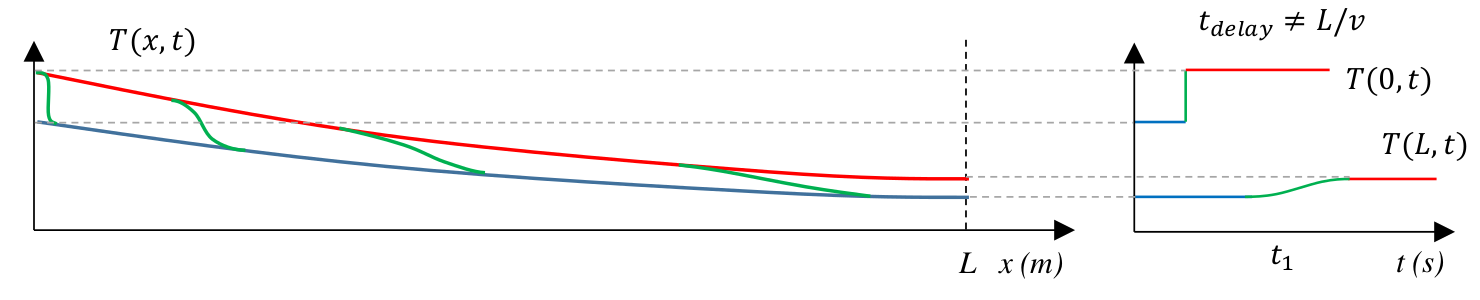
\includegraphics[width=\textwidth]{figures/heat_front}
  \caption{Proces šíření teplotní vlny v potrubí}
\end{figure}

Parciální diferenciální rovnice (PDR) pro celkovou dynamiku je pak v tomto
kontextu následující:
\begin{equation}
  \label{eq:AdvDiff}
  \frac{dy}{dt} = -u \frac{dy}{dx} + D\frac{d^{2}y}{dx^2} + {S_y}
\end{equation}
kde \(y\) je unášená veličina, \(t\) je čas, \(x\) je podélná poloha, \(u\) je
rychlost tekutiny, \(D\) je celkový koeficient difúze a \(S_y\) je celkový
zdroj unášené veličiny. Z hlediska tepelného chování může být touto veličinou
měrná entalpie, ale lze pracovat i s teplotou.

\begin{itemize}
  \item
    \textbf{Advekce} je jev, při kterém se transportují veličiny (jsou unášeny)
    ve směru objemového pohybu. Tento jev ovlivňuje tepelnou dynamiku nejvíce,
    neboť z velké části určuje čas transportu (zpoždění) teplotní fronty.
  \item
    \textbf{Axiální difúze} je složena jednak z difúze kondukcí tepla v
    tekutině a dále z tzv. turbulentního míchání v axiálním směru. Difúze
    způsobená kondukcí je u teplárenských rozvodů zanedbatelná
    \cite{VanderHeijde2017a,VanderHeijde2017b}. Za to turbulentní difúze roste
    přibližně lineárně s Reynoldsovým číslem \cite{Chertkov2018}. Axiální
    difúze způsobuje rozpínání (vyhlazování) teplotní fronty, což znamená,
    že náhlé změny na vstupu do potrubí se projevují pozvolnými změnami na jeho
    konci. V případě uvažování horizontálně uloženého potrubí lze tímto
    způsobem zahrnout i vliv gravitace. Axiální difúze nemá vliv na zpoždění
    teplotní fronty, ale výrazně ovlivňuje její tvar.
  \item
    \textbf{Zdrojový termín} \(S_y\) zahrnuje především výměnu tepla mezi
    tekutinou a vnitřním povrchem přilehlé stěny ve kterém tekutina proudí (což
    v důsledku určuje vliv akumulace tepla na vývoj teplotní fronty). Velikost
    hustoty tepelného toku je závislá na rozdílu teploty vody a povrchu,
    vlastnostech tekutiny, velikosti a drsnosti povrchu a na rychlosti
    proudění. Výměna tepla ovlivňuje jak zpoždění teplotní fronty tak její
    tvar. Tuto intenzitu lze vyjádřit rovnicí pro konvekci tepla
    \ref{eq:ConvHeatTransfer}.
\end{itemize}

\begin{equation}
  \label{eq:ConvHeatTransfer}
  Q = \alpha S \Delta T
\end{equation}
kde \(Q\) je tepelný tok ze stěny do tekutiny, \(\alpha\) je součinitel přestupu
tepla, \(S\) je velikost plochy styčného povrchu a \(\Delta T\) je rozdíl
teplot povrchu a tekutiny. Koeficient přenosu tepla  je možné určovat z
tzv. Nusseltova čísla, které vyjadřuje poměr mezi konvektivním a koduktivním
přestupem tepla. Známe-li tedy množství tepla, jež by procházelo mezní vrstvou
v případě čisté kondukce tepla je možné určit množství tepla v případě
konvektivního přestupu tepla:

\begin{equation}
  \label{eq:NusseltDef}
  Nu = \frac{\alpha L}{\lambda}
\end{equation}
kde je \(Nu\) Nusseltovo číslo, \(L\) je charakteristický rozměr (pro kruhové
potrubí je jím vnitřní průměr) a \(\lambda\) je tepelná vodivost tekutiny.

\begin{figure}[h] \centering \capstart
  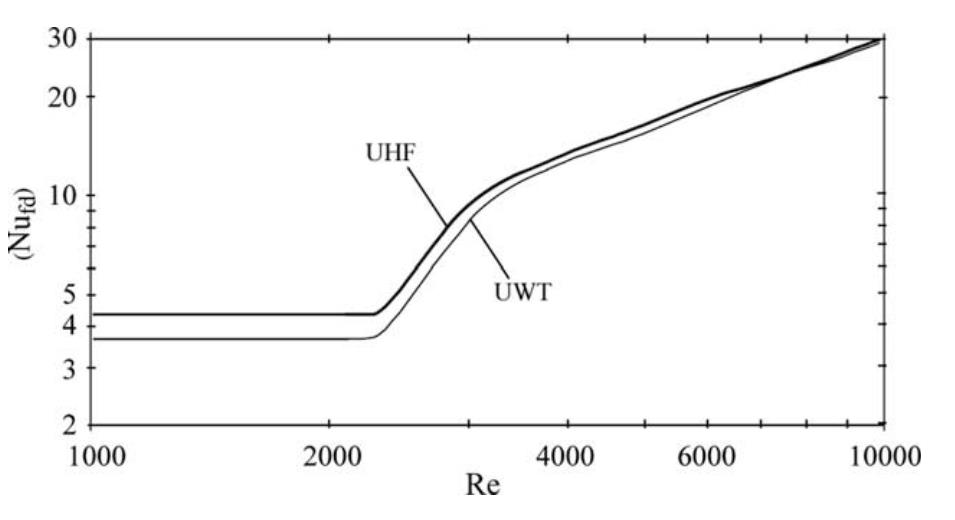
\includegraphics[scale=0.3]{figures/nusselt}
  \caption{Závislost Nusseltova čísla na Reynoldsově čísle \cite{Abraham2009}}
  \label{fig:NuReynolds}
\end{figure}

Hodnotu Nusseltova čísla je možné určit na základě vztahů jak pro rovnoměrné
rozložení teploty na stěně (označováno jako UWT), tak pro rovnoměrné rozložení
tepelného toku (označované jako UHF). Dle \cite{Abraham2009} je pro všechny
režimy proudění vhodné používat následující model Nusseltova čísla:
\begin{equation}
\label{eq:NuModel}
  Nu =
  \begin{dcases}
    c_0 & Re\leq 2300 \\
    \sum_{i=1}^{5} c_i\left(\frac{Re}{10^3}\right)^{5-i} & 2300 < Re\le 3100 \\
    \frac{\frac{f}{8}(Re-1000)Pr}
    {1+12.7{\frac{f}{8}}^{(1/2)}(Pr^{(2/3)}-1)} & 3100 < Re
  \end{dcases}
\end{equation}
kde \(Pr\) je Prandtlovo číslo (vlastnost tekutiny) a \(f\) je Darcy-Weisbachův
koeficient tření, který je popsán v podkapitole \ref{sec:PressureLoss} (skrze
něj se projevuje vliv drsnosti). Jednotlivé hodnoty parametrů tohoto modelu
jsou:
\begin{table}[H]
  \label{tab:NuModel}
  \caption{Parametry modelu Nusseltova čísla}
  \vskip
  \centering
  \begin{tabular}{ccc}
    \toprule
    Parametr & UWT & UHF \\ [0.5ex]
    \hline
    \(c_0\) & 3,66 & 4,36 \\
    \(c_1\) & 3,52 & 2,2407 \\
    \(c_2\) & 45,148 & 29,499 \\
    \(c_3\) & 212,13 & 142,32 \\
    \(c_4\) & 427,45 & 292,51 \\
    \(c_5\) & 316,08 & 219,88 \\
    \bottomrule \\[0.1mm]
  \end{tabular}
\end{table}
V případě, že je teplota vnitřního povrchu potrubí známa je možné na základě
rovnic \ref{eq:ConvHeatTransfer} až \ref{eq:NuModel} určit intenzitu výměny
tepla v konkrétním okamžiku. Teplota tohoto povrchu je však ovlivněna tepelnou
hmotou jež obklopuje fluidní region (např. ocelová trubka, izolace, zemina
pod.) a tudíž je nutno korektně matematicky zachytit tepelnou dynamiku v tomto
okolí (viz~kapitola \ref{sec:SurroundingMass}).

\section{Fluidní region - tlakové ztráty/akcelerace tekutiny}
\label{sec:PressureLoss}
Tlakové vlny se v potrubí šíří výrazně rychleji (rychlostí zvuku) než vlny
teplotní (přibližně rychlost proudění tekutiny), což znamená, že lokální
události probíhají v daleko kratším časovém měřítku. Z tohoto důvodu je potřeba
v simulacích s tlakovými pulsacemi využívat krátký časový krok. Predikce
tlakových vln je užitečná pouze z hlediska ochrany proti poškozením, která
jsou způsobena tlakovými rázy a na vývoj distribuce tepla nemá výraznější vliv.
Při zanedbání rychlých tlakových pulsací lze akceleraci tekutiny podél potrubí
modelovat pomocí PDR \ref{eq:momentum}. Výsledné chování je ekvivalentní k
okamžitému šíření informací o tlaku do celého systému.

\begin{equation}
  \label{eq:momentum}
  \frac{du}{dt}\rho = -\frac{dp}{dx} - \frac{1}{2}\frac{f}{D}u|u|
\end{equation}
kde \(p\) je tlak a \(D\) je vnitřní průměr potrubí. Hodnotu třecího
koeficientu \(f\) lze určit z explicitní Churchilovy rovnice \ref{eq:Churchill}
\cite{Churchill1977}, která je relativně přesná pro všechny režimy proudění.

\begin{equation}
  \label{eq:Churchill}
  \begin{gathered}
    f=8\left(\left(\frac{8}{Re}\right)^{12}+(A+B)^{-1.5}\right)^\frac{1}{12} \\
    A=\left(2.457\ln\left(\left(\frac{7}{Re}\right)^{0.9}
      +0.27\frac{\epsilon}{D}\right)^{-1}\right)^{16} \\
    B=\left(\frac{37530}{Re}\right)^{16}
  \end{gathered}
\end{equation}
kde \(\epsilon\) je drsnost vnitřního povrchu potrubí a \(D\) je vnitřní průměr
potrubí.

\section{Okolní hmota – kovová stěna, izolace, zemina}
\label{sec:SurroundingMass}
Pro popis vedení tepla v okolí fluidního regionu potrubí je vhodné využít
obecnou PDR vedení tepla \ref{eq:HeatEq} v obecném \(\mathcal{R}^n\) prostoru.
\begin{equation}
  \label{eq:HeatEq}
  \frac{dT}{dt}\rho{c_p}=\nabla(\lambda\nabla{T})+S
\end{equation}
kde \(\rho\) je hustota, \(c_p\) je měrná tepelná kapacita, \(\lambda\) je
tepelná vodivost, \(T\) je teplota a \(S\) je zdroj tepla. Tato rovnice platí
pro všechny souřadnicové systémy, jelikož pro každý souřadnicový systém
existuje konkrétní varianta operátoru \(\nabla\). Dále je třeba uvažovat
okrajové podmínky zajišťující interakci s dalším okolím.
\begin{itemize}
  \item
    \textbf{Okrajové podmínky pro nadzemní potrubí} musí reflektovat interakci
    vnějšího povrchu rozvodů s okolním vzduchem. Dle aktuálních povětrnostních
    podmínek se tedy jedná o přenos tepla přirozenou či nucenou
    konvekcí tepla. Jde tedy o okrajovou podmínku třetího řádu (Robinovu).
  \item
    \textbf{Okrajové podmínky pro podzemní potrubí} musí reflektovat jak
    interakci s prostředím, které se nachází nad povrchem země (to může být
    samotný vzduch nebo městská infrastruktura, budovy apod.) tak s dostatečně
    vzdálenou zeminou jak v horizontálním tak vertikálním směru. Jedná se tedy
    o tři různé okrajové podmínky. Dle \cite{danielewicz2016172} je nevhodnější
    použít okrajovou podmínku prvého řádu (Dirichletovu) pro spodní okraj
    uvažované domény a podmínky druhého řádu (Neumannovu) pro oba její
    vertikální okraje. Okrajová podmínka na horním okraji je pak řádu třetího
    podobně jako u nadzemního potrubí nebo řádu čtvrtého v případě přítomnosti
    městské infrastruktury (z hlediska numerického řešení jsou si podmínky
    třetího a čtvrtého řádu velmi podobné).
\end{itemize}

\begin{figure}[!tbph]
  \centering
  \begin{minipage}{.35\textwidth}
    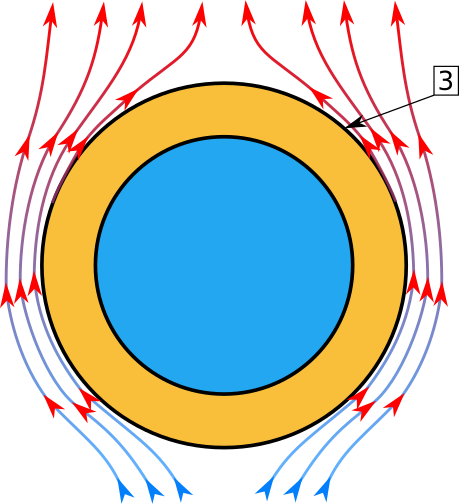
\includegraphics[width=\textwidth]{figures/above_ground_pipe}
    \caption{Nadzemní potrubí}
    \label{fig:above_ground_pipe}
  \end{minipage}
  \begin{minipage}{.50\textwidth}
    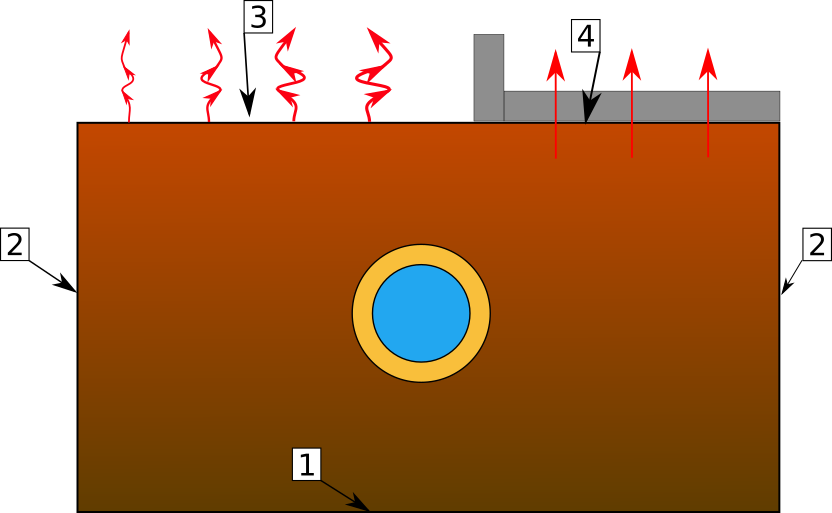
\includegraphics[width=\textwidth]{figures/burried_pipe}
    \caption{Podzemní potrubí}
    \label{fig:burried_pipe}
    \end{minipage}
\end{figure}
\section{Vlastnosti média a materiálu}
Vlastnosti tekutiny a materiálů jež vystupují v rovnicích \ref{eq:AdvDiff} až
\ref{eq:HeatEq} jsou ve skutečnosti závislé na teplotě a na tlaku (nebo
obecněji na stavových veličinách). Existují implementace programů mezinárodní
asociace pro vlastnosti vody a páry (IAPWS) \cite{IAPWS2007}, které popisují
vlastnosti vody a páry velmi přesně. Při uvažování nestlačitelnosti vody jsou
vlastnosti jako hustota, či viskozita stále výrazně proměnlivé s teplotou. Pro
tuhé skupenství je zpravidla dostačující popis polynomiální funkcí nebo i
konstantou. Při popisu zeminy se může výrazně projevit vliv její vlhkosti, což
znamená, že její vlastnosti jsou proměnlivé v čase.

\begin{figure}[h] \centering \capstart
  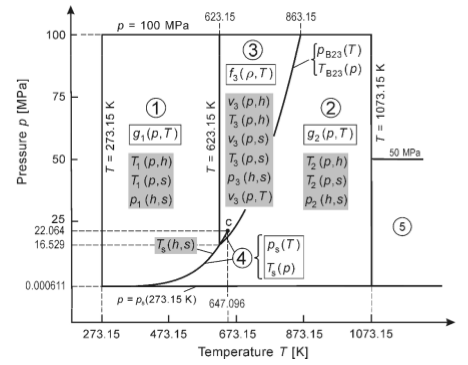
\includegraphics[scale=0.4]{figures/IF97}
  \caption{Regiony implementace vlastností vody a páry IF97 \cite{IAPWS2007}}
  \label{fig:IF97}
\end{figure}

\section{Numerické řešení a rychlost simulací}
\label{sec:NumSpeed}
V rovnicích \ref{eq:AdvDiff}, \ref{eq:momentum} a \ref{eq:HeatEq} vystupují
diferenciální operátory, jež jsou fundamentální příčinou numerické náročnosti
simulací. I přesto, že je fyzika popsaná v sekcích \ref{sec:HeatDynamics},
\ref{sec:PressureLoss} a \ref{sec:SurroundingMass} výrazně zjednodušena, je
tyto PDR nutné diskretizovat v prostoru a čase (tzv. linearizovat problém). Lze
využít metody jež jsou určeny a optimalizovány přímo pro daný kontext.
Například pro rovnici \ref{eq:AdvDiff} lze využít integrační metody vyvinuté v
NASA, které využívají aproximace derivací vyšších řádů, nežli je v samotné PDR.
Takové řešení lze nalézt např. v \cite{leonard1988}, kde jedním z
nejefektivnějších schémat je ULTIMATE QUICKEST.

Avšak mnohem častější postup při řešení PDR je její převedení na systém
ordinárních diferenciálních rovnic (ODR), jež je dále integrován (simulován) v
čase pomocí separátních algoritmů. PDR jsou v prostoru nejčastěji linearizovány
pomocí metody konečných diferencí (MKD), metody konečných objemů (MKO) či
metod konečných prvků (MKP). Pro sestavení matic a následnou integraci v čase
existuje celá řada komerčních nástrojů s přednastavenými řešiči pro jednotlivé
systémy PDR. Z Open-Source projektů zabývajícími se automatizovaným řešení PDR
je vhodné zmínit FeniCS \cite{AlnaesBlechta2015a}, kterým je možné řešit PDR
pomocí MKP (umožňuje i tzv. nespojitou Galerkinovu metodu, která je vhodná i
pro fluidní dynamiku). Tato knihovna umožňuje velmi detailně kontrolovat jakým
způsobem jsou sestavovány matice, jaké konečné elementy jsou využívány, jakým
způsobem bude během výpočtů manipulováno s objekty lineární algebry a mnoho
dalšího.

Výsledkem procesu linearizace je systém lineárních rovnic z pravidla
reprezentovaný v maticové formě. Velikost a hustota (podíl nenulových hodnot)
těchto matic pak přímo ovlivňují rychlost simulace, neboť přímo korespondují s
počtem CPU cyklů, které musí procesor (či procesory) využít na aritmetické
operace během jednoho časového kroku. V případě, že je výsledný systém
nelineární (např. jsou-li tepelné vlastnosti závislé na teplotě) je tento vliv
ještě umocněn. Pro integraci v čase existují explicitní či implicitní algoritmy
s konstantním nebo adaptivním časovým krokem. Jedny z nejefektivnějších
algoritmů jsou součástí knihovny SUNDIALS \cite{sundials}, která je
implementována v jazyce C.

\section{Vliv programovacích jazyků na modelování procesů}
\label{sec:proglang}
Programovací jazyky využité v jednotlivých modulech simulací mohou výrazně
ovlivnit výpočtovou rychlost.
\begin{itemize}
  \item
    \textbf{Kompilované jazyky} jako jsou C, C++ či Fortran jsou zpravidla
    jedny z nejrychlejších, avšak za cenu náročnějšího často velmi
    nízkoúrovňového programovaní. Tato náročnost je způsobena faktem, že tyto
    jazyky (zejména jazyk C), jsou ''mnohem~blíže'' hardwaru. Programátor musí
    například staticky určit všechny typy proměnných a také zabezpečit, že
    nedojde k nesprávnému přístupu do paměti počítače.
  \item
    \textbf{Interpretované jazyky} jako Python či Matlab jsou z hlediska
    programovaní mnohem jednodušší protože poskytují výrazně vyšší úroveň
    abstrakce a existuje k nim velké množství modulů a knihoven. Úkol spojený s
    hlídáním datových typů proměnných a správnosti přístupů do paměti počítače
    zajišťuje tzv. interpretr (interpretr pro Python je zkompilovaný C program
    zvaný CPython) a programátor má výrazně ''jednodušší život'', protože se
    může soustředit pouze na vysokoúrovňový koncept výpočtů. Programy (nebo
    přesněji skripty) napsané v těchto jazycích jsou však kvůli práci
    interpetru až o dva řády pomalejší o proti svým kompilovaným protějškům.
  \item
    Nový \textbf{Just-in-time kompilovaný jazyk} Julia \cite{julia2017}
    dosahuje rychlosti srovnatelné s jazykem C, ale zároveň poskytuje velmi
    vysokou úroveň abstrakce. Jednotlivé varianty funkcí (určeno dle typu
    argumentů, které vstupují do funkce) jsou průběžně kompilovány. Julia
    udržuje v paměti, které verze jsou již zkompilovány a které nikoliv.
    To znamená, že každé další použití již zkompilované varianty se bude chovat
    velmi podobně jako běžný kompilovaný objekt a čas potřebný na interpretaci
    v tomto okamžiku již není relevantní. Nevýhoda jazyku Julia oproti výše
    zmíněným interpretovaným jazykům spočívá v jeho novosti, což znamená, že
    mnoho vysokoúrovňových knihoven neexistuje nebo nejsou ve stavu ve kterém
    se na ně lze spoléhat.
\end{itemize}
Další relevantní dělení programovacích paradigmatů je z hlediska řízení pořadí
jednotlivých operací (instrukcí).
\begin{itemize}
\item
\textbf{Imperativní} programovací jazyky (všechny jež jsou zmíněny výše), mění
stav programu přesně dle programátorem definované sekvence. Programy jsou
spouštěny z výchozího bodu a běží přesně definovaným směrem.
\item
\textbf{Deklarativní} programovací jazyky využívají paradigmatu ve kterém
programátor definuje logické a matematické výroky mezi objekty a konkrétní
výpočtové posloupnosti jsou vytvářeny počítačem (kompilerem). To znamená, že
programy nemají přesně definovaný výchozí bod a mohou být z principu spouštěny
libovolným směrem a z různých stavů. Jeden z takových jazyků je například
modelica, který byl vyvinut pro matematické modelování systémů složených z
interagujících komponent. OpenModelica \cite{Fritzson2019} je open-source verze
kompilátoru, který překládá modely ze syntaxe modelica do imperativních jazyků
(např. jazyka C) a automaticky linkuje vůči knihovnám jako jsou právě SUNDIALS
z kapitoly \ref{sec:NumSpeed}. Standardní knihovna modelica (MSL) také obsahuje
implementaci vlastností vody dle standardu IF97 (standart IAPWS). Simulace jsou
pak relativně rychlé a také velmi modulární. Pro nezasvěceného se může
deklarativní programování jevit poněkud krkolomné, ale po překonání této
bariéry je tento styl programování často schůdnější (zejména u komponentami
orientovaných simulací).
\end{itemize}
Obecně tedy nejde o to, který programovací jazyk je nejlepší, ale spíše o
jejich spojení tak, aby spolu jednotlivé moduly dobře spolupracovali a
programátor se vyhnul zbytečnému nízkoúrovňovému programování v situacích kde
by nepřineslo dostatečné výhody.
\section{Komplexní distribuční systém}
\label{sec:Complex_distr_sys}
Matematické modely systémů jež jsou složené z mnoha komponent (zde myšleno jak
matematických tak fyzikálních abstrakcí) mohou být z hlediska komplementace
značnou výzvou. Zejména zde se projevují výhody deklarativního jazyka jako je
modelica. Jednotlivé naprogramované komponenty je možné propojovat a vnořovat
do sebe bez nutnosti detailního popisu pořadí výpočtových instrukcí. OMC by měl
v budoucnosti poskytovat možnosti pro kompilaci modelů s automatickou
parallelizací. Pro paralelizaci systémů se značnou numerickou komplexností lze
využít open-source kosimulačního standardu zvaného \textit{functional mock-up
interface} (FMI). V případě zásobování teplem by to např. znamenalo propojení
simulací městských oblastí tedy jedné \textit{functional mock-up unit} (FMU),
kde je každá oblast simulována na jiné části hardwaru a FMI standard poskytuje
výměnu nezbytných proměnných mezi těmito modely tak aby byla zajištěna jejich
správná interakce.

\section{Počítačové učení a jeho vztah k modelování procesů}
\label{sec:ML}
\begin{figure}[h] \centering \capstart
  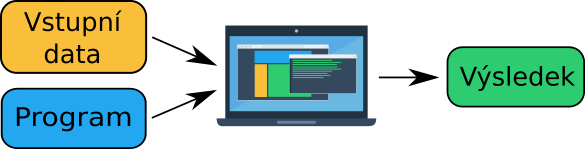
\includegraphics[scale=0.6]{figures/traditional_prog_cz}
  \caption{Tradiční programování}
  \label{fig:traditional_prog}
\end{figure}

\begin{figure}[h] \centering \capstart
  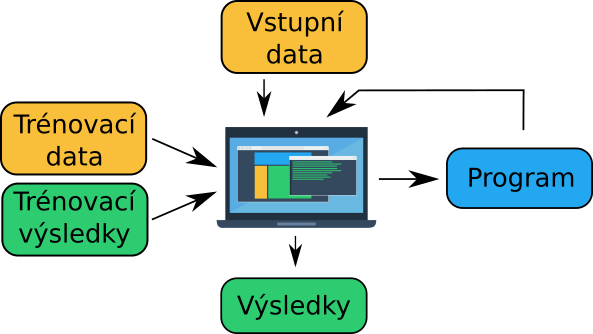
\includegraphics[scale=0.6]{figures/machine_learning_cz}
  \caption{Počítačové učení}
  \label{fig:machine_learning}
\end{figure}
Počítačové učení (anglicky machine learning) je metoda tvorby programů. Jedná
se o postup kdy je program (nebo jeho část) vytvořen počítačem. Tato oblast se
dále dělí na následující oblasti:
\begin{itemize}
  \item
    \textbf{Supervised learning} je metoda učení, která využívá člověkem
    přiřazené výsledky ke vstupním trénovacím datům. Typickým příkladem je
    klasifikace na základě znaků v datech. Trénovací data obsahují člověkem
    vytvořené anotace s požadovanými výsledky.
  \item
    \textbf{Unsupervised learning} je metoda kdy nejsou data nijak označena,
    ale algoritmus odhaluje klíčové znaky samostatně bez pomoci člověka.
    Typickým příkladem je autoenkódování.
  \item
    \textbf{Reinforcement learning} je metoda kdy prostředí ve kterém program
    operuje poskytuje informace o dopadu zásahů tohoto programu na dané
    prostředí. Typickým příkladem může být řídící člen (agent) v simulaci.
\end{itemize}
Programy v machine learning jsou v podstatě
parametrizované matematické struktury a optimalizací jejich parametrů je možné
měnit/zlepšovat chování programu. Tyto programy dále obsahují tzv.
hyperparametry, kterými se řídí struktura a komplexnost programů.

Poměrně velký úspěch v této oblasti zaznamenaly tzv. neuronové sítě (NN). Jsou
totiž velmi univerzálními aproximátory matematických funkcí, což je jejich
velkou výhodou. Jejich nevýhodou je naopak poměrně náročný proces učení a také
fakt, že vyžadují poměrně velké množství dat.

Nedávno (2019) se objevily vědecké práce, které navrhují a demonstrují využití
NN (nebo obecně parametrizovaných programů) pro matematické modelování ODR
systémů (a tudíž i PDR) \cite{diffEqFlux2019,chen2018neural}. Ukázkové modely
byly v těchto dvou implementacích prováděny akcelerovanou metodou gradient
descend, přičemž gradient byl určen algoritmickou zpětnou propagací skrze ODR
solver (což je největším přínosem těchto prací). Gradient descend je obecně
považován za nejvíce pokročilou metodu učení modelů, avšak je poměrně náročný
na implementaci.

Existují i algoritmy jež nevyžadují derivace a jsou vhodné pro modely, u
kterých nelze derivace určit. Tyto algoritmy umožňují optimalizaci až na úrovni
black box. Více o těchto algoritmech lze nalézt v kap. \ref{sec:opt_alg}.

Machine learning a mechanistické modelování na základě PDR lze tedy kombinovat.
Tímto je možné modelovat procesy na základě experimentálních dat, zjednodušovat
komplexnost programů na základě extrahovaných veličin z více komplexních
simulací nebo optimalizovat (ladit) známé mechanistické struktury pomocí
experimentálních dat.

\section{Optimalizační algoritmy nultého řádu}
\label{sec:opt_alg}
Optimalizační algoritmy tzv. nultého řádu jsou i v dnešní době předmětem
aktivního výzkumu. Například \cite{golovin2019gradientless} nabízí čerstvý
pohled na využití Gausovské vzorkování jakožto klíčové metaheuristiky pro
tzv. \textit{gradientless descend} (GLD). Mezi pokročilé techniky takového
typu optimalizace patří evoluční strategie (zde je velmi známá metoda
využívající adaptace kovarianční matice definující vzorkovací prostor)
\cite{hansen2016cma}, genetické algoritmy, náhodná hledání či stochastická hledání.
Tyto algoritmy nebývají deterministické právě proto, že zpravidla využívají
generátory náhodných čísel. Jejich úkolem je nalézt minimum či maximum funkce o
níž není známa její gradient. Jediná hodnota která je pro takový algoritmus
přístupná je hodnota tzv. účelové funkce, což je hodnota popisující vhodnost či
nevhodnost jednotlivých řešení. Například při optimalizaci založené na
jednoduché mutaci (evoluční strategie) se pro pokusná řešení využívá slovo
vzorek. Tyto vzorky jsou konstruovány během tzv. epoch (nebo generací). Každá
epocha začíná s určitým množstvím vzorků, jež jsou během epochy zhodnoceny a na
základě těchto výsledků jsou vygenerovány nové vzorky pro další epochu.
Meteheuristika evoluční strategie je proces, který manipuluje se vzorkovacím
prostorem tak aby se zvýšila pravděpodobnost, že v následující epoše budou
nalezeny lepší vzorky než v epoše předcházející. Tímto postupně nalézáme lepší
a lepší řešení daného optimalizačního problému, dokud není nalezeno nejlepší
možné řešení (může dojít k nalezení pouze tzv. lokálního optima). Jednotlivé
strategie jsou vhodné jen pro určité problémy a proto jsou optimalizační
nástroje zpravidla vybaveny celou sadou různých algoritmů.
\chapter{Shrnutí vybraných studií}
itext

\chapter{Analýza, interpretace a zhodnocení poznatků}
itext
\chapter{Podstata, cíle a přínos disertační práce}
\label{chap:Aims_of_disertation}
\section{Podstata disertační práce}
\label{sec:Podstata}
Podstatou této disertační práce je výzkum možností využití počítačového učení
v oblasti matematické modelování fyzikálních procesů komponent a systémů
složeného z těchto komponent se zaměřením na CZT. V principu jde tedy o
modelování PDR. Jedná se o základní výzkum zaměřený na optimalizaci
numerických výpočtů/simulací využívající distribuované strojové vybavení.
Jeho řešení spočívá ve vytvoření optimalizačního nástroje s aplikačními
rozhraními umožňující jeho propojení s matematickými modely/simulacemi
implementovanými v různých programovacích jazycích tak, aby bylo možné
zlepšovat jejich efektivitu a/či přesnost nebo modelovat/zachycovat procesy s
nedokonale objasněnými fyzikálními mechanismy s pomocí experimentálních dat.
\section{Cíle práce}
\label{sec:Aims}
Cílem disertační práce je vytvořit nástroje pro optimalizaci parametrizovaných
programů, propojit je s matematickými modely komponent (a systémů) a
demonstrovat jeho funkčnost pro modely CZT. Optimalizační nástroj (s pracovním
názvem LOFI) bude schopen optimalizovat parametry jak mechanistických tak
neuronových modelů. Cílovými veličinami mohou být jak experimentální data, ale
také data z komplexnějších simulací nebo penalizační účelové funkce (například
v případě optimalizace řídících veličin).
\begin{itemize}
  \item
    Vytvořit nástroje pro optimalizaci parametrizovaných programů (simulací).
  \item
    Propojit tyto nástroje s modely komponent CZT a demostrovat jejich
    funkčnost.
\end{itemize}
\subsection*{Jednotlivé kroky}
\begin{itemize}
  \item
    Sestavení a naprogramování modulárního modelu advektivně-difúzivní
    mechaniky pro fluidní region teplárenských rozvodů s přestupem tepla do
    okolí.
  \item
    Sestavení parametrizovaného modelu akumulace tepla do okolí teplárenských
    rozvodů.
  \item
    Naprogramovaní optimizátorů v jazyce Python schopných běhu na počítačových
    clusterech splňující Unix standartazaci (Linux). Pro komunikaci
    jednotlivých uzlů bude využit uzlový komunikační protokol MPI. Ohled bude
    brán i na minimalizaci síťové komunikace také pomalých I/O přístupů
    například pomocí ukládání do paměti RAM.
  \item
    Pro snadnější implementaci výše zmíněného bude navržen jednoduchý plánovač
    úloh s příhodnými funkcemi (využívající zejména MPI) pro efektivní saturaci
    uzlů clusteru.
  \item
    Naprogramovaní aplikačního rozhraní na OMC pro snadné propojení
    optimizátoru s matematickými modely implementovanými v
    \textbf{deklarativním} jazyce modelica.
  \item
    Sestavení modelu menšího teplárenského systému a optimalizace řídících
    veličin.
\end{itemize}
\section{Přínos disertační práce}
\label{sec:prinos}
Hlavní přínos práce je v oblasti základního výzkumu. Navrhované postupy a
nástroje mohou výrazně usnadnit hledaní řídících strategií s ohledem na
integraci fluktuicích nízkoteplotních zdrojů a také usnadnit hledání
optimalních matematických modelů komponent ze kterých, je vhodné sestavit model
většího systémů. Navrhovaný postup a nástroje pro optimalizaci modelů mohou být
následně využity i mimo oblast CZT, jejichž vývojem se na našem pracovišti
taktéž intenzivně zabýváme.

\chapter{Vědecké otázky a pracovní hypotézy}
\label{chap:SciQaH}
\subsection*{Vědecká otázka č. 1}
Jakou strukturu mají matematické modely teplárenských rozvodů, ze kterých lze
snadno sestavit vetší potrubní systém a které reflektují akumulaci tepla do
okolního materiálu a zároveň lze optimalizovat jejich numerické schopnosti?
\subsection*{Hypotéza č. 1}
Je možné sestavit ekvivalentní tepelné schéma radiálního šíření tepla o
příslušné komplexnosti a optimalizovat jeho parametry tak aby model dosahoval
co největší shody s plně disktretizovaným 2D protějškem, přičemž fluidní
region je modelován pomocí jednorozměrné advektivně-difúzivní mechaniky. Tímto
může být dosaženo výrazné redukce komplexnosti při zachování dostatečné
přesnosti.
\subsection*{Vědecká otázka č. 2}
Jak optimalizovat řídící veličiny teplárenského systému v rámci dlouhodobých
horizontů z hlediska ekonomicky či účinnosti?
\subsection*{Hypotéza č. 2}
V čase rozmístěné řídící veličiny mohou být optimalizovány na základě simulací,
které obsahují data o předpovědi počasí (nebo obecně předpovědi venkovních
vlivů) kde skutečné řídící veličiny jsou interpolovány z diskrétních okamžiků.
Tyto diskrétní body je pak nutné holisticky optimalizovat.
\subsection*{Vědecká otázka č. 3}
Jak přistupovat k problému optimalizace dynamických modelů reprezentovanými
systémy ODR nebo systémem diferenciálními algebraických rovnic (např. výše
zmíněné tepelné schéma)?
\subsection*{Hypotéza č. 3}
Nejpraktičtější je využití optimizátoru jež nevyžaduje první derivace vůči
parametrům modelu (tzn. nultého řádu, např. evolučních strategie), protože
odpadá problém s poměrně složitým výpočtem těchto derivací. Modely pak mohou
být implementovánv v jazyce modelica nebo obecně jiném programovacím prostředí.
Takovým přístup je možné optimalizovat obecně modely i řídící parametry.
\chapter{Způsob řešení a použité vědecké metody zkoumání}
Tato kapitola se věnuje způsobům a metodám řešení aplikovaných v jednotlivých
vytyčených cílech.
\section{Jednodimenzionální model potrubí}
\label{sec:1Dpipe}
V programovacím jazyce modelica bude sestavena komponenta fluidního regionu
potrubí s parametrizovaným advektivním schématem druhého nebo třetího řádu pro
rozumnou minimalizaci numerické difúze ostré teplotní vlny (podobně jako v
metodě QUICKEST) a také jednoduché schéma prvého řádu pro skutečnou fyzikální
difúzi. Model výměny tepla mezi tekutinou a vnitřním povrchem bude
implementován dle \cite{Abraham2009} s třecím koeficient dle
\cite{Churchill1977}. Parametry modelu Nusseltova čísla mohou být následně
optimalizovány pro daný kontext. Model bude obsahovat rozhraní pro spárování s
modelem akumulace tepla.
\begin{figure}[h]
\begin{center}
  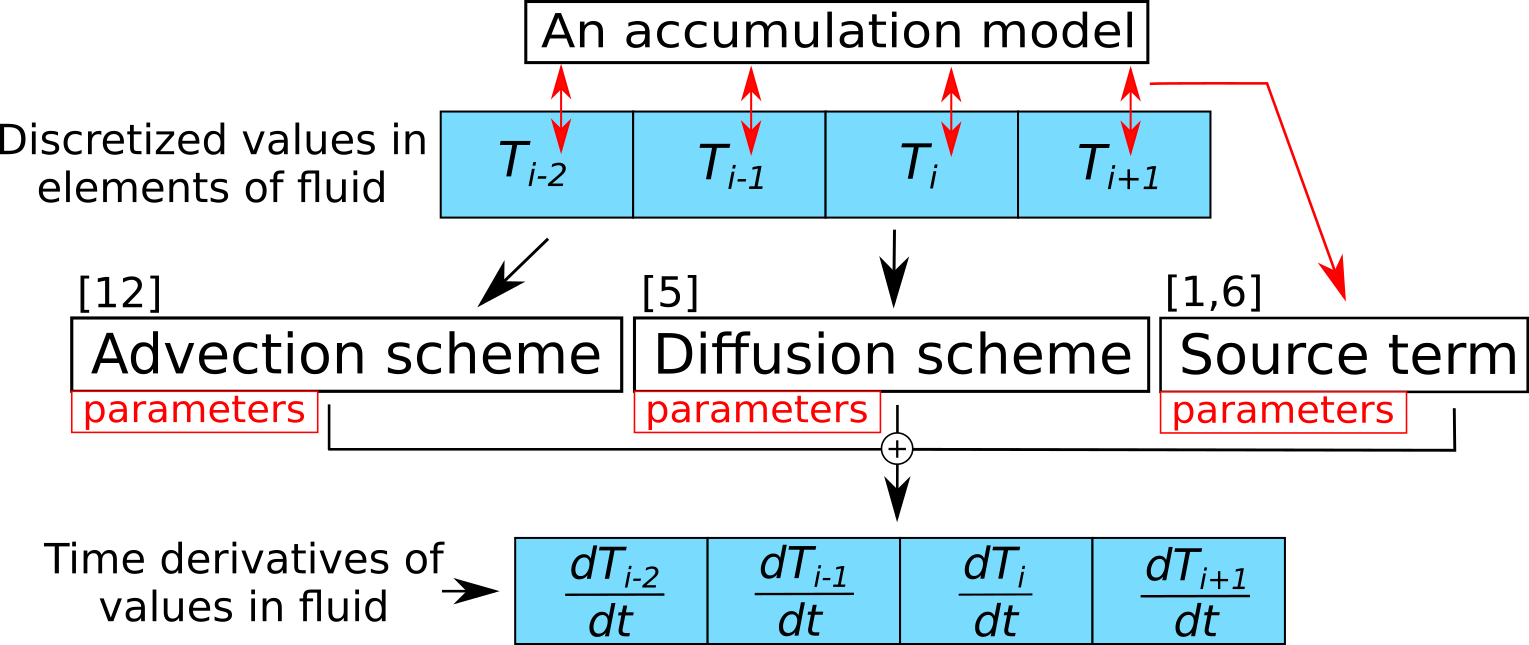
\includegraphics[scale=0.9]{figures/1D_model_pipe}
\end{center}
\caption{Model fluidního regionu}
\label{fig:pipe_model}
\end{figure}

\section{Model akumulace tepla v okolí potrubí}
\label{sec:PipeAcu}
Pro nadzemní potrubí bude v jazyce modelica sestaven model reflektující
tepelnou dynamiku jednotlivých válcových vrstev (ocel, izolace apod.). Model
bude založen na MPK se specificky navrženými konečnými elementy. Pro
podzemní potrubí bude nejdříve sestavena komplexní dvourozměrný model pomocí
metody MKP. K tomuto účelu bude využit nástroj FeniCS. Na základě dat z těchto
simulací bude chování modelu přeneseno optimalizací stupňů volnosti (pomocí
LOFI) do zjednodušeného ekvivalentního schématu naprogramovaného v jazyce
modelica (a kompilovaného pomocí OMC). Přidáváním, odebíráním a změnou
topologie schématu je možné měnit chování zjednodušeného modelu (přesnost a
numerická efektivita). Tyto modely akumulace budou obsahovat rozhraní pro
spárování s modelem fluidního regionu a případně i vlivy okolí. 
\begin{figure}[h]
\begin{center}
  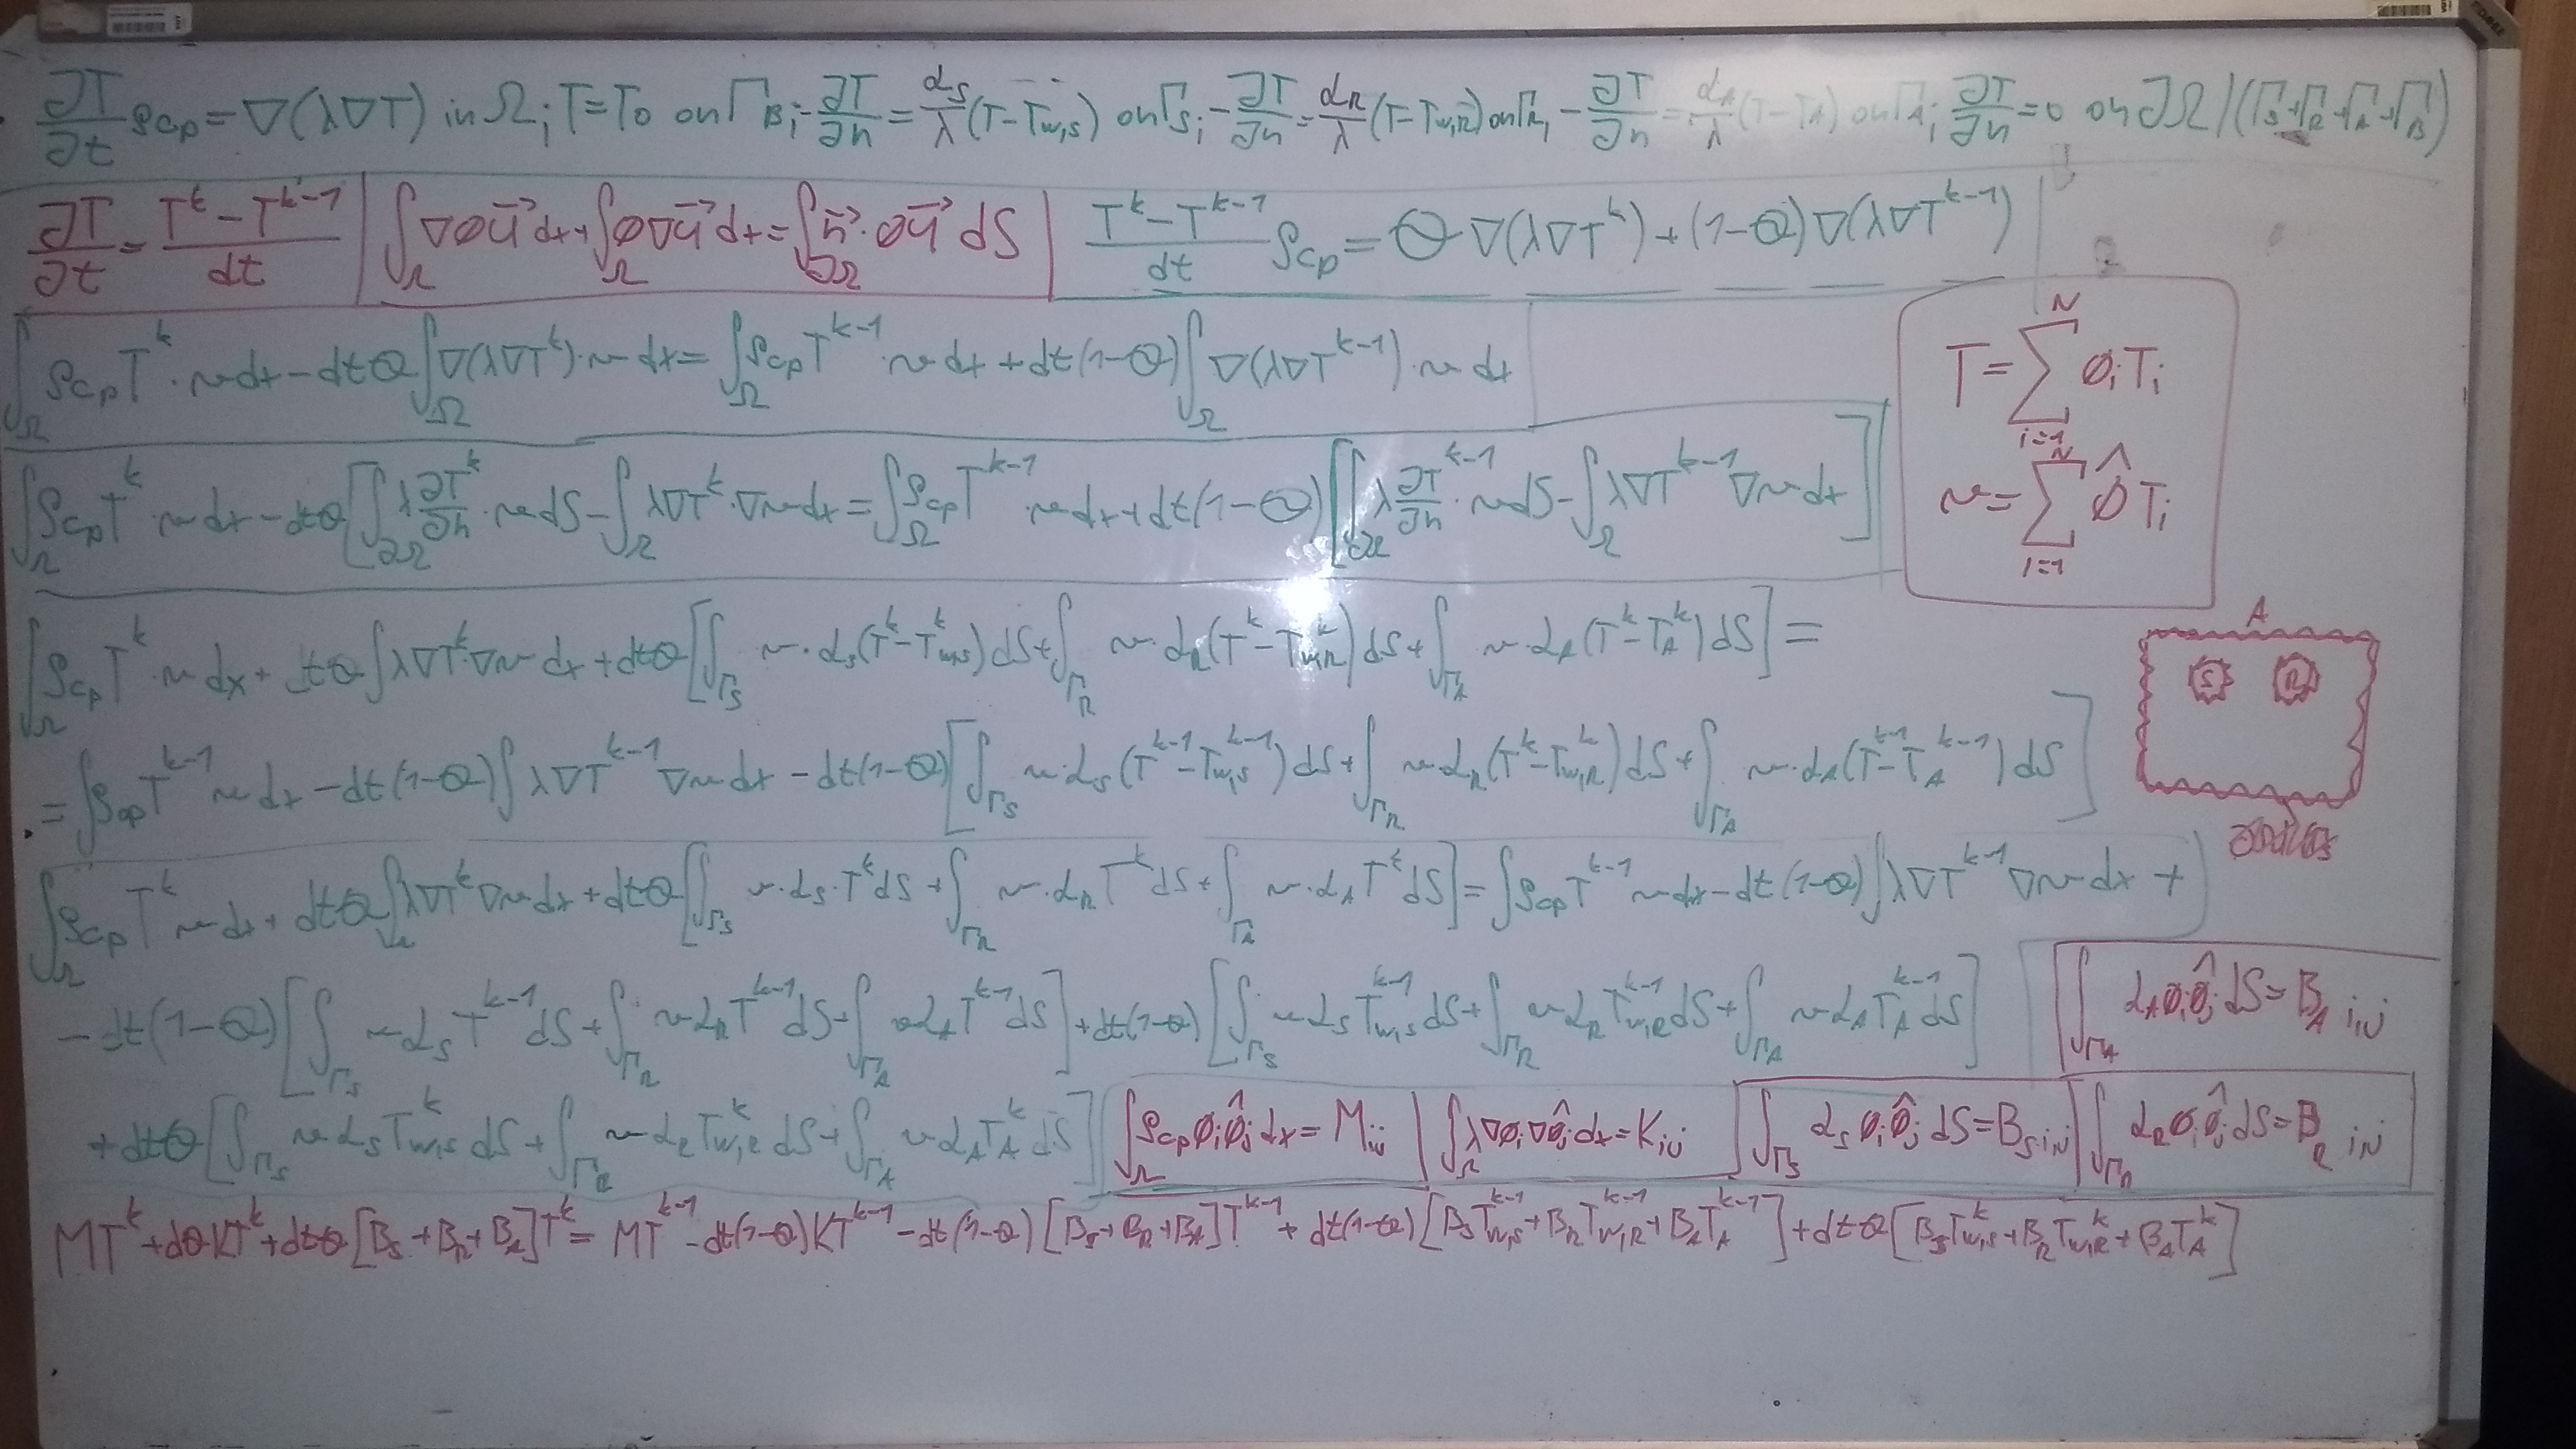
\includegraphics[scale=0.09]{figures/Assembly_TimeDependent}
\end{center}
\caption{Symbolická linearizace PDR vedení tepla v okolí potrubí pomocí MKP}
\label{fig:VariationalMathTwoPipes}
\end{figure}
\begin{figure}[h]
  \centering
    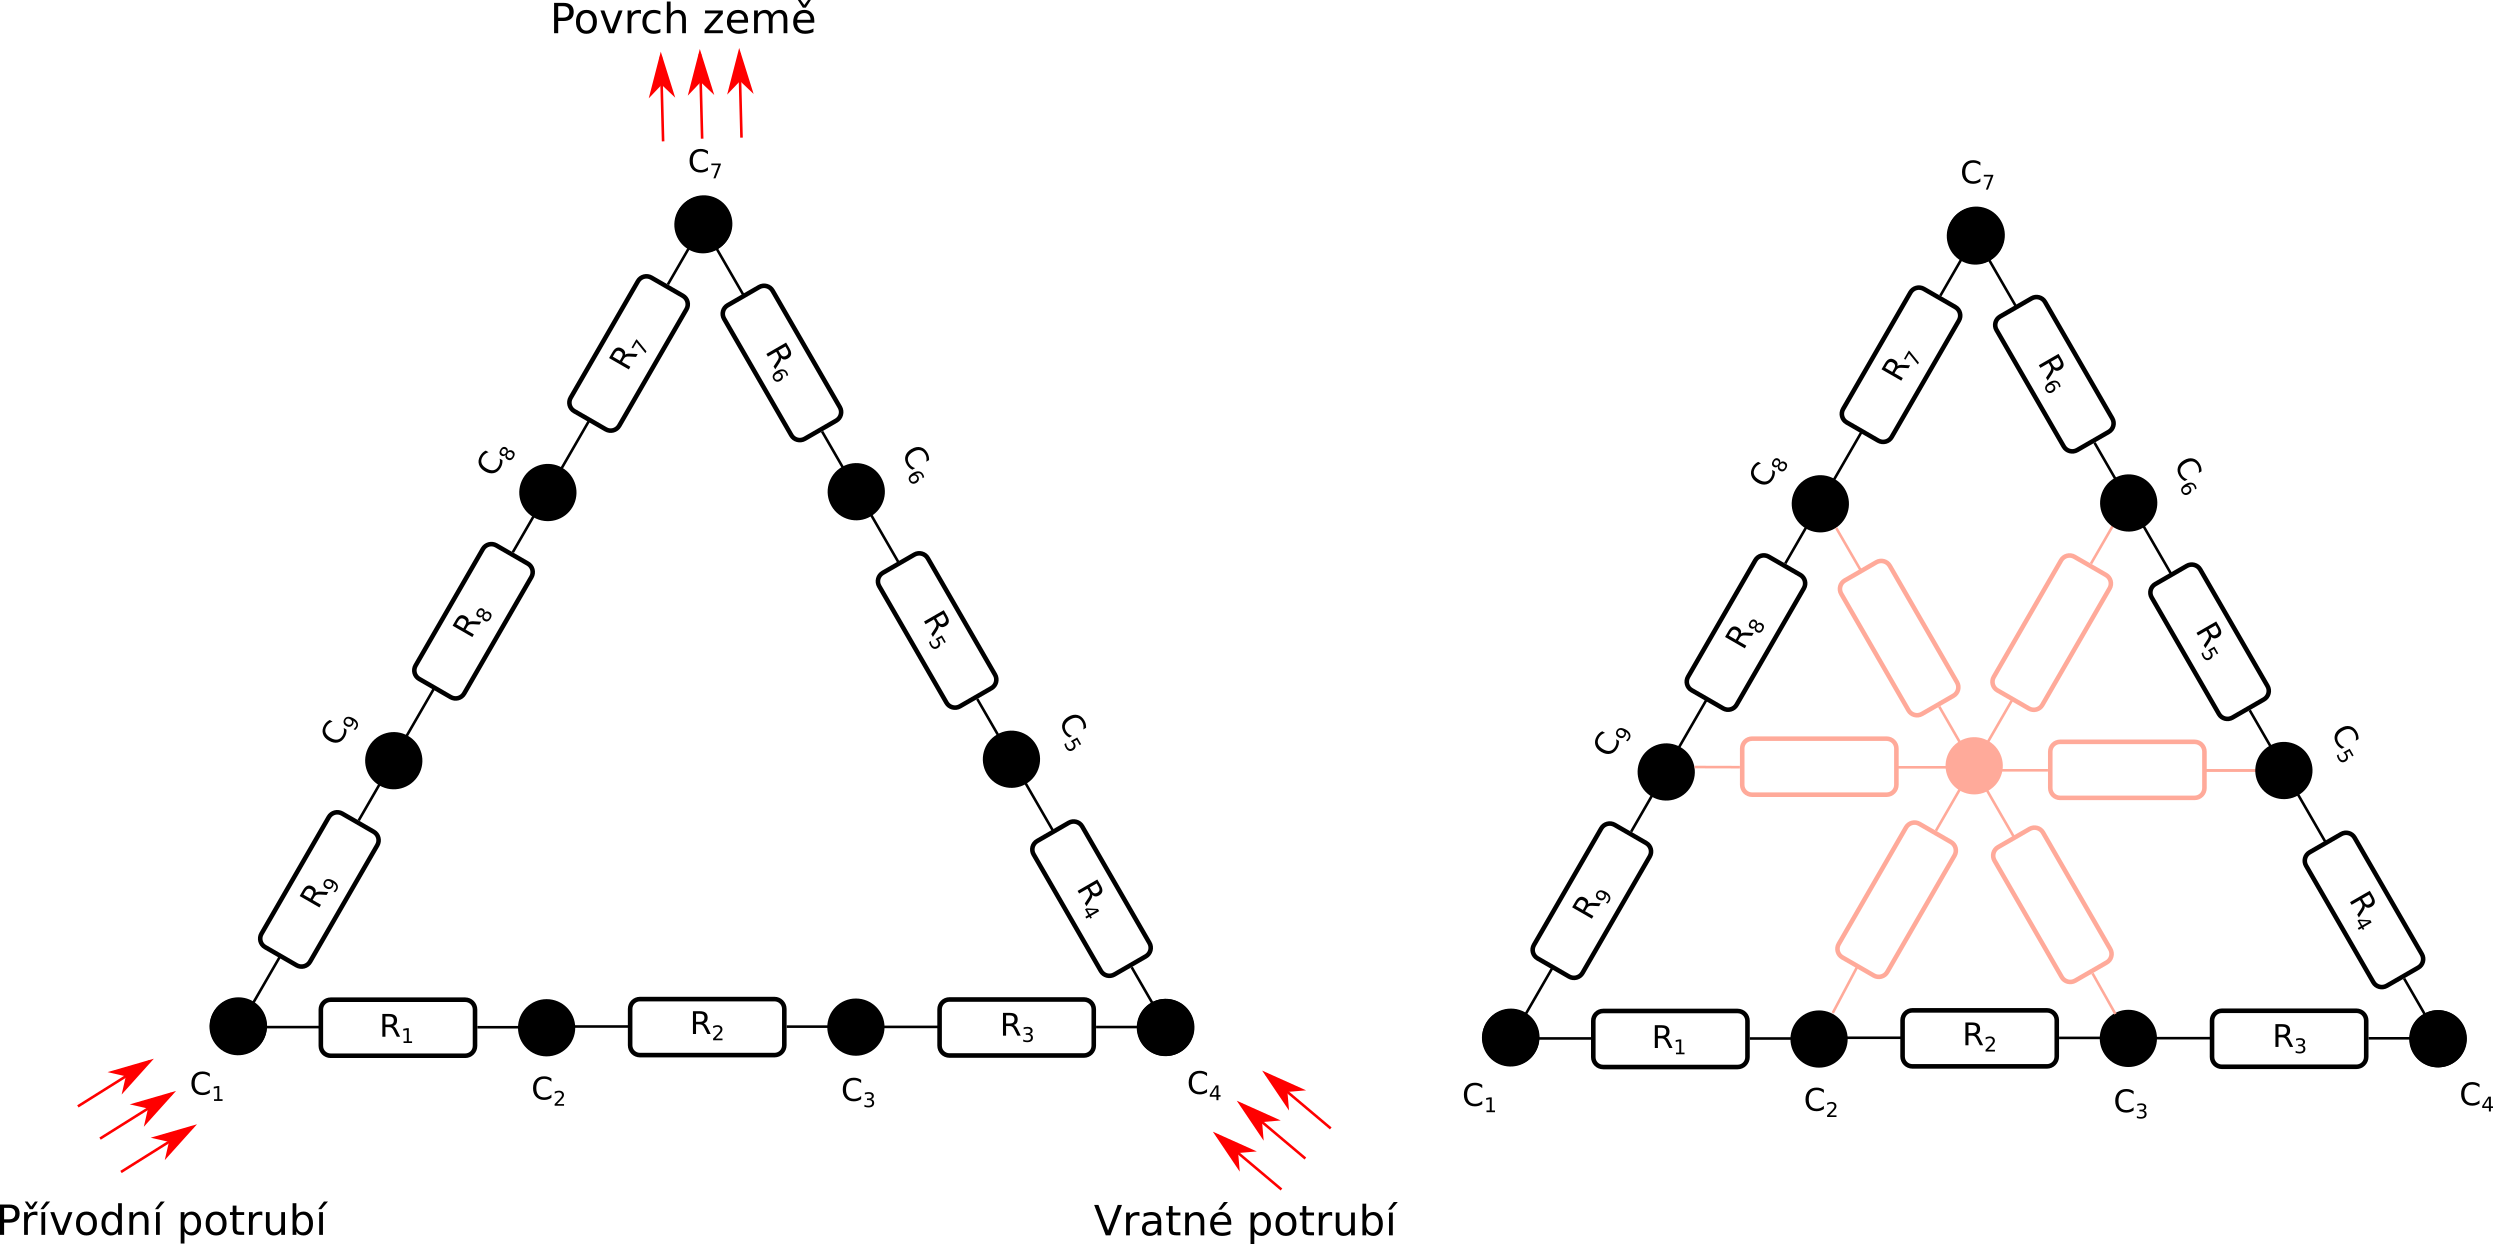
\includegraphics[width=0.75\textwidth]{figures/acumulation_burried}
    \caption{Ekvivalentní tepelné schémata vedení tepla v zemině (nalevo
      základní schéma, napravo schéma s více stupni volnosti)}
    \label{fig:above_ground_pipe}
\end{figure}
\section{Nástroj LOFI}
\label{sec:tool_LOFI}
Při řešení bude sestaven optimalizační nástroj LOFI (nejedná se o zkratku, ale
pouze o dočasné jméno), který bude obsahovat aplikační rozhraní zejména k OMC.
Nástroj bude implementován v jazyce Python. Bude obsahovat paralelizované verze
evolučních strategií, hejnových algoritmů, klesání v bloku souřadnic apod.
Jelikož se předpokládá, že pro některé parametry budou modely simulací
produkovat neočekávané chování, nebo tzv. \textit{floating-point exceptions} či
budou kompletně neschopné běhu, bude zapotřebí zajistit dostatečná opatření
zvyšující pravděpodobnost optimalizace i za takto náročných podmínek. Pro
paralellizaci na clusterech bude využito knihoven MPI se zaměřením na Unixové
systémy. Architektura bude založená na tzv. \textit{master-worker} paradigmatu.
Protože modely zkompilované pomocí OMC produkují výsledky do binárních souborů,
které se ukládají na disk, bude využit RAMdisk (kterým je Linuxový kernel
zpravidla vybaven) pro akceleraci I/O přístupů a také ochranu hardwaru. LOFI
bude obsahovat dynamický plánovač úloh pro maximální saturaci clusteru
simulacemi. LOFI bude také schopno operovat v interaktivním režimu pomocí
integrované konzole schopné vnitřně komunikovat s ostatními uzly clusteru.
\begin{figure}[h]
\begin{center}
  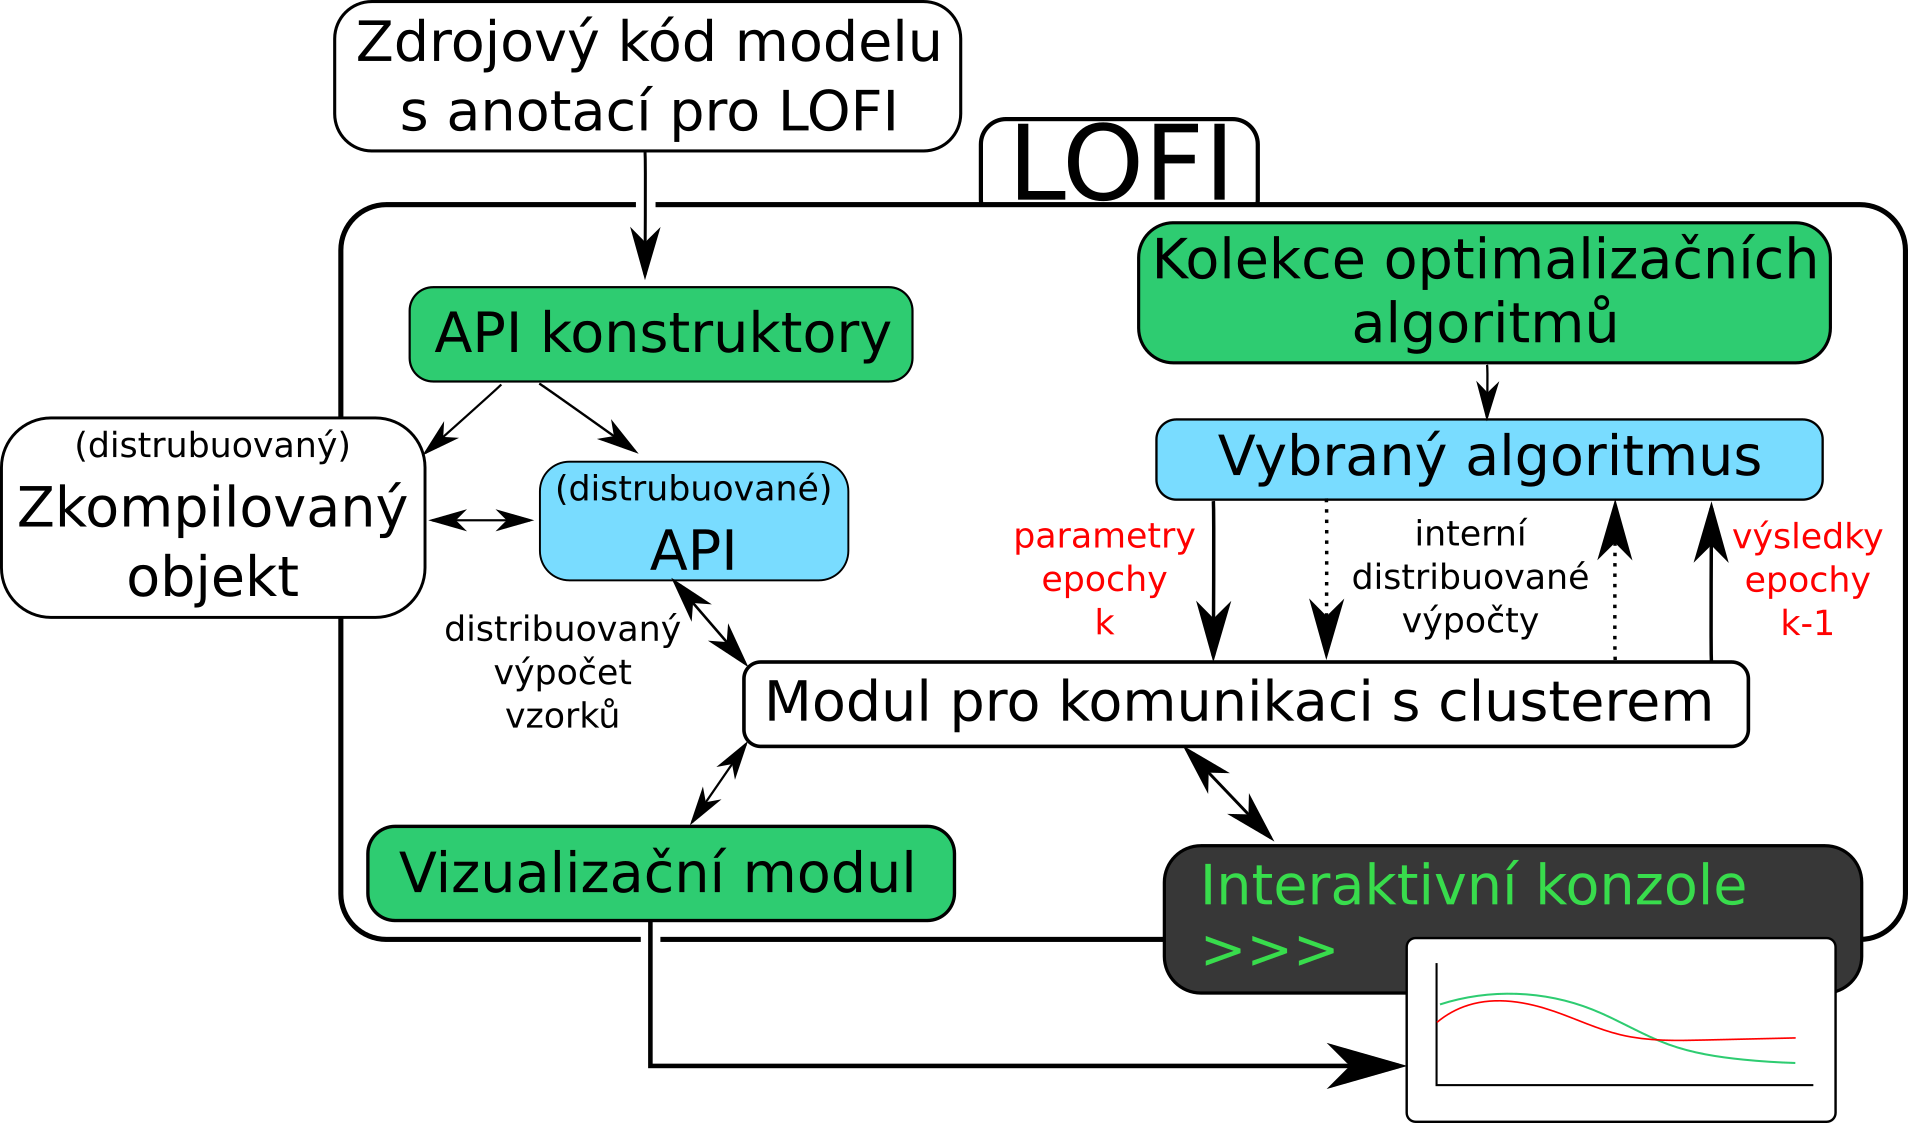
\includegraphics[scale=0.5]{figures/LofiArchitecture}
\end{center}
\caption{Optimalizační nástroj LOFI}
\label{fig:LOFI}
\end{figure}

\section{Prediktivní řízení}
\label{sec:MPC}
LOFI bude v poslední fázi použito pro optimalizaci základních řídících
parametrů sítě. Po sestavení malého teplárenského systému z jednotlivých
komponent bude do modelu zahrnuta časová distribuce řídících veličina jako jsou
teplota vstupní vody či průtok u zdroje.
\section{Dosavadní dosažené výsledky}
\label{sec:Finished_parts}
\subsection{Fluidní region rozvodů a akumlace v nadzemním potrubí}
V roce 2019 byl publikován článek \cite{Kudela2019pipe}, ve kterém je popsán
matematický model nadzemního potrubí s akumulací. Je zde popsán matematický
model fluidního regionu. Model je založen na výše popsané metodice, ale není
optimalizován nástrojem LOFI. Optimalizace probíhala pomocí generátoru schémat
a následným výběrem nejefektivnějšího schématu na základě vybraných kritérií
jako je míra numerické difúze či nefyzikální oscilace. Výsledný differenciální
operátor pro advekci je druhého řádu a je z části podobný schématu QUICKEST.
Model se vyznačuje dobrou numerickou účinností v porovnání s nástroji
\textit{ANSYS Fluent} či \textit{\mbox{STAR-CCM+}} přičemž vykazuje velmi
dobrou shodu ve výsledném řešení šíření teplotní fronty. V~tomto článku je
porovnáno a zhodnoceno mnoho dalších potenciálních vlivů na simulaci. Je zde
také obsaženo odvození tvarových funkcí pro variační model akumulace do válcové
stěny založené na stacionárním řešení.
\begin{figure}[h]
  \begin{center}
    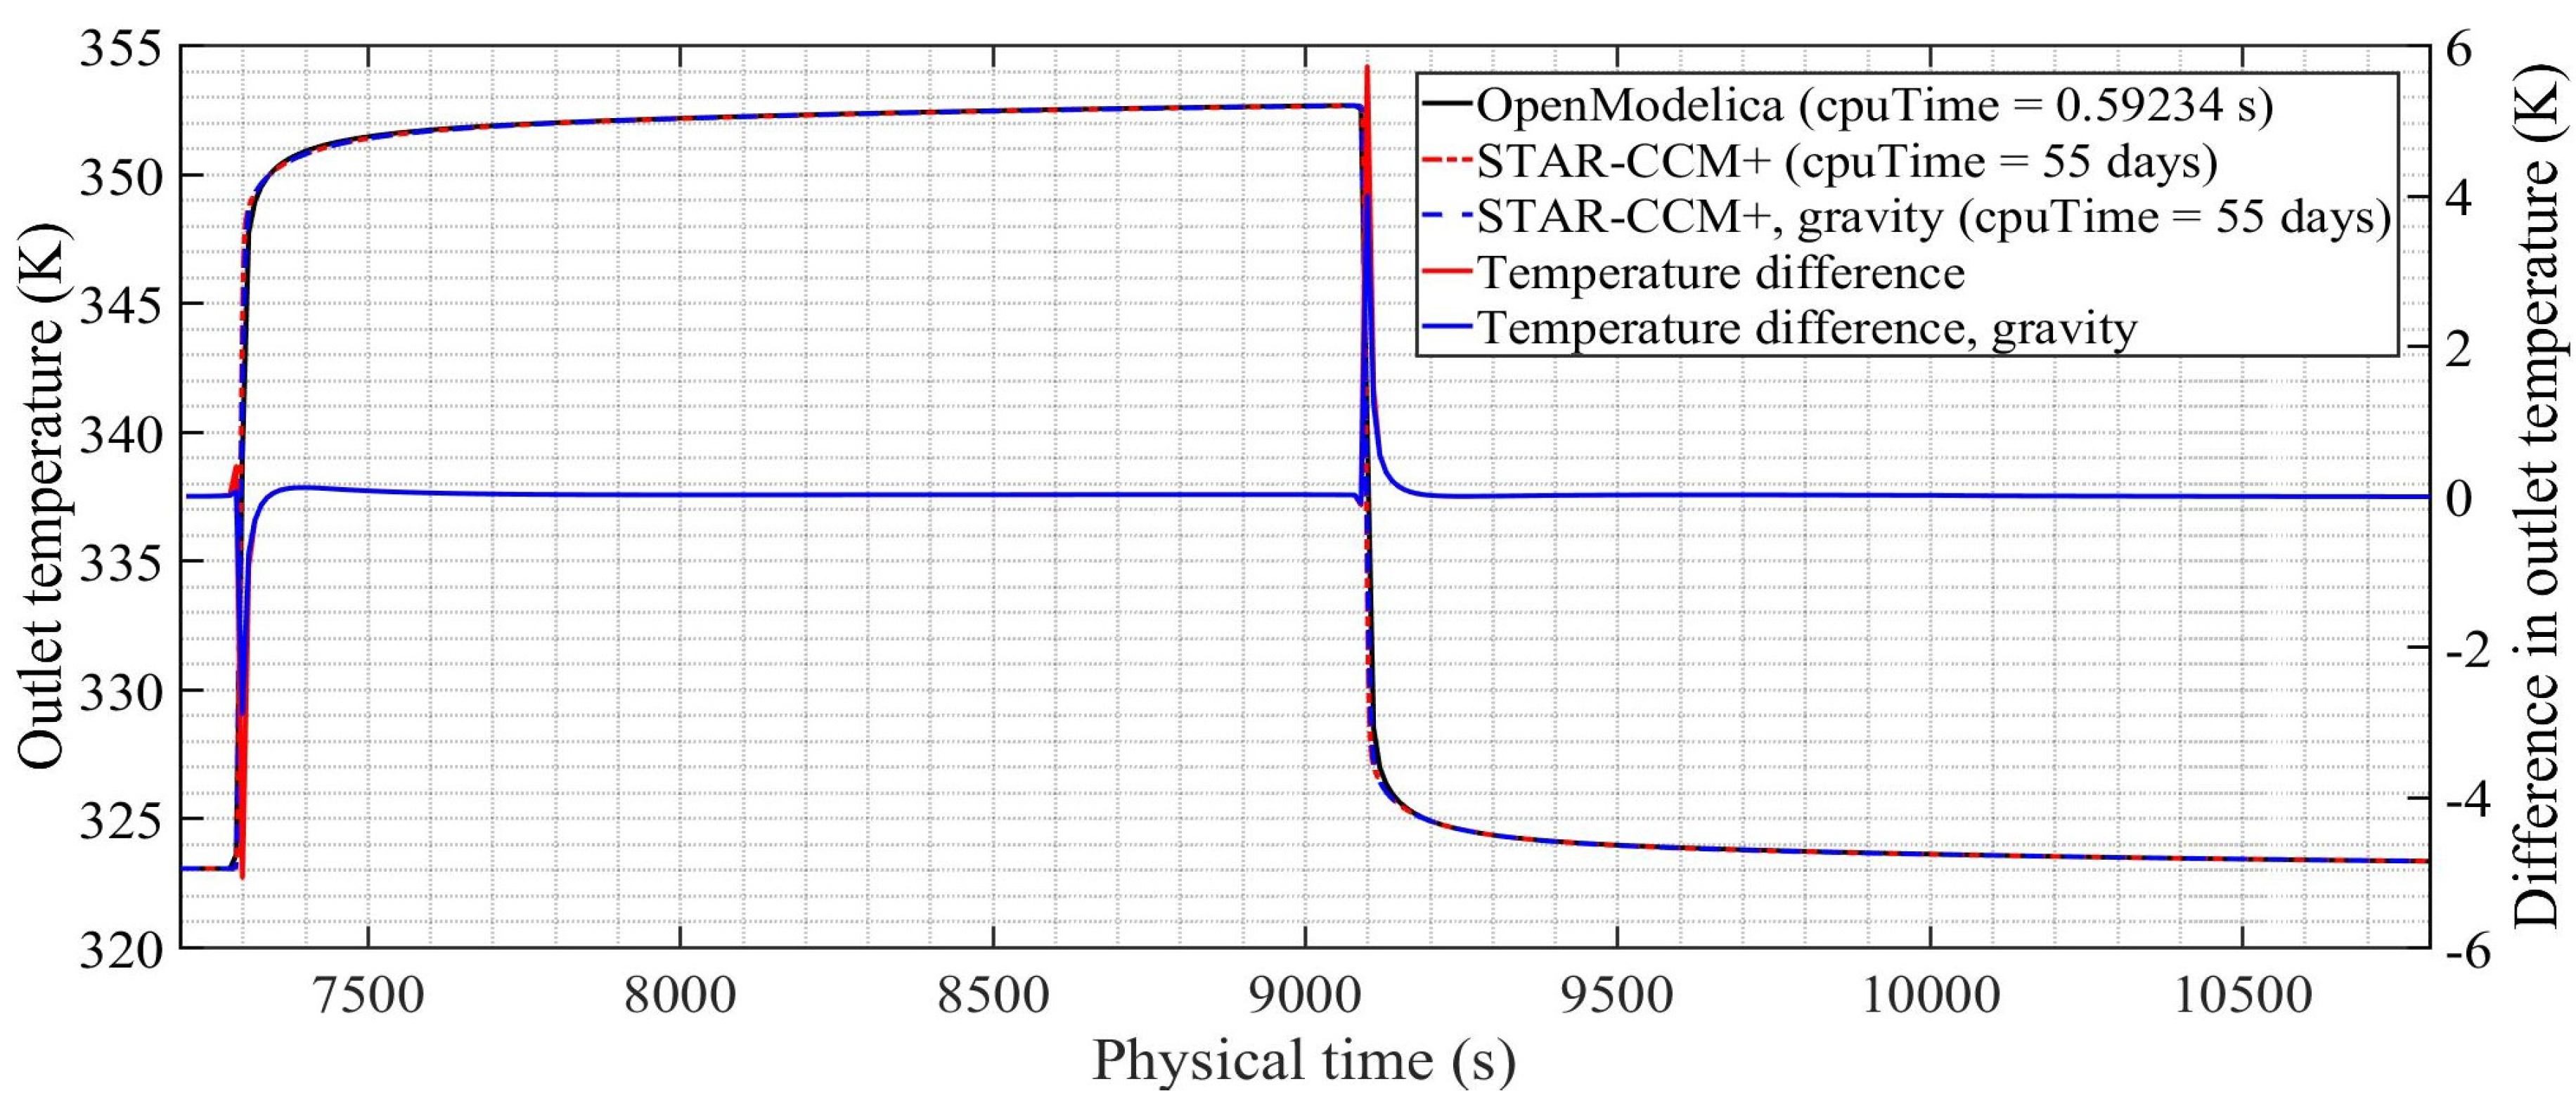
\includegraphics[scale=0.7]{figures/pipe_CCM_OM}
  \end{center}
  \caption{Srovnání nového modelu se simulací ve STAR-CCM+}
  \label{fig:}
\end{figure}
\begin{figure}[h]
  \begin{center}
    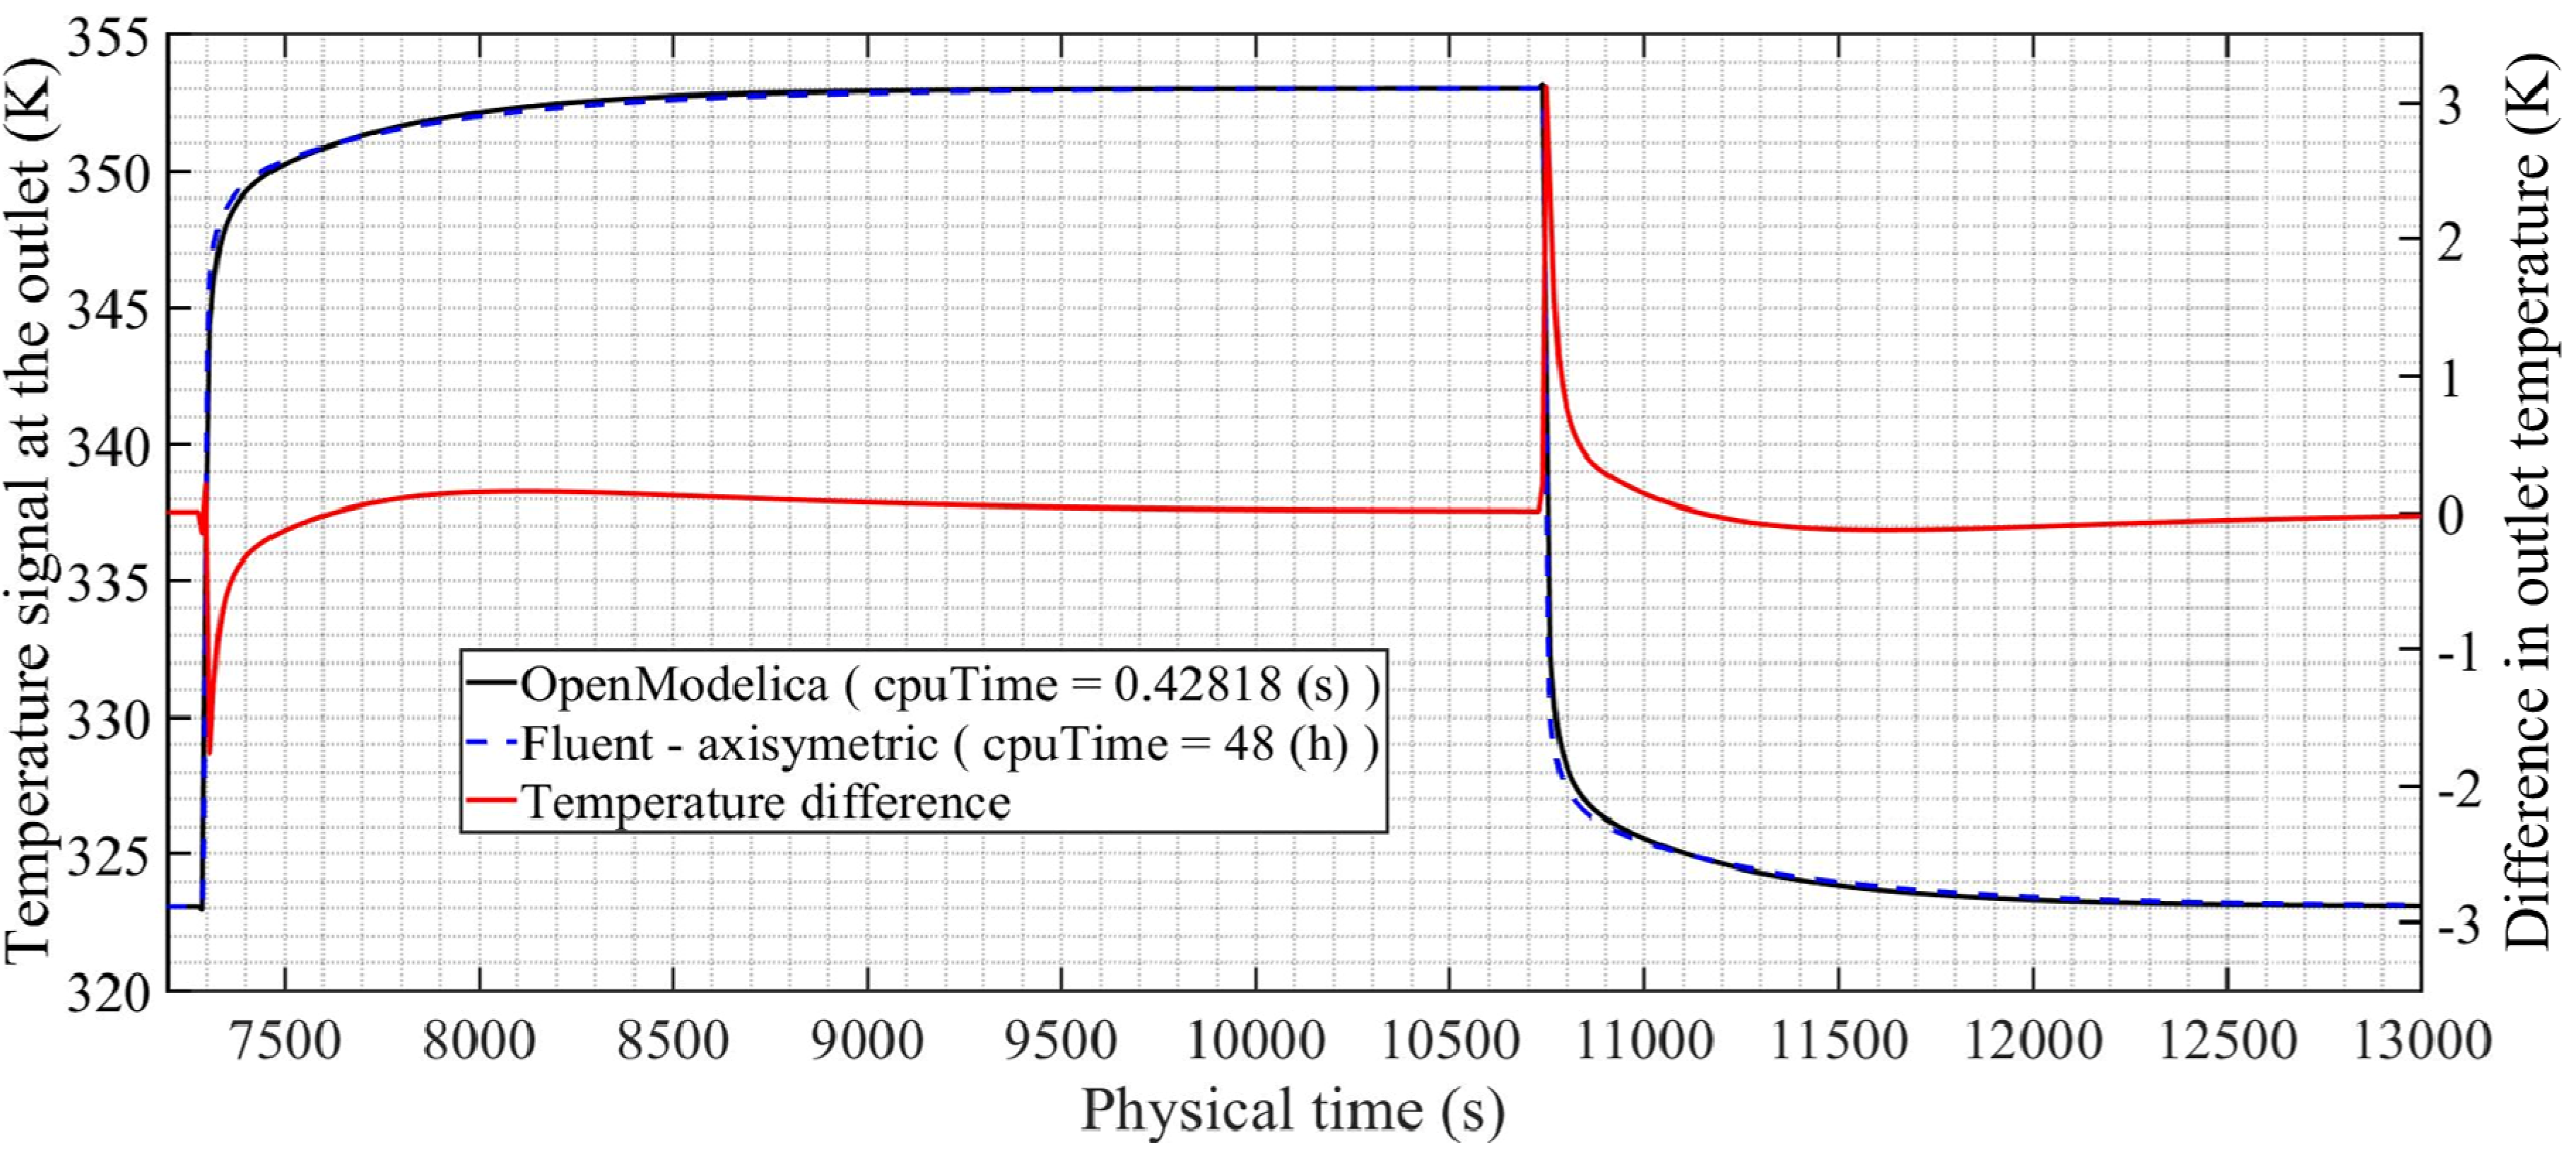
\includegraphics[scale=0.7]{figures/pipe_Fluent_OM}
  \end{center}
  \caption{Srovnání nového modelu se simulací v ANSYS Fluent}
  \label{fig:}
\end{figure}
\subsection{Komplexní model akumulace tepla v zemině}
V programovacím jazyce python byl sestaven efektivní nástroj pro simulaci 2D
řezů rozvodů potrubí zejména s využitím knihovny mshr a FeniCS. Nástroj na
základě parametrů automaticky sestaví síť, vytvoří příslušné řídké matice
(paralelizace probíhá na úrovní lineární algebry) a simuluje data pomocí
integrační metody druhého řádu (Crank-Nicolson). Pro akceleraci výpočtu se
během méně dynamického průběhu je využito adaptace časového kroku pomocí odhadu
chyby v zákonu zachování energie. Tento model je vhodný i pro simulace tzv.
twinpipe rozvodů. Optimalizace zjednodušeného schématu (převod dynamiky z
komplexní simulace) zatím nebyla otestována.

\begin{figure}[h]
\begin{center}
  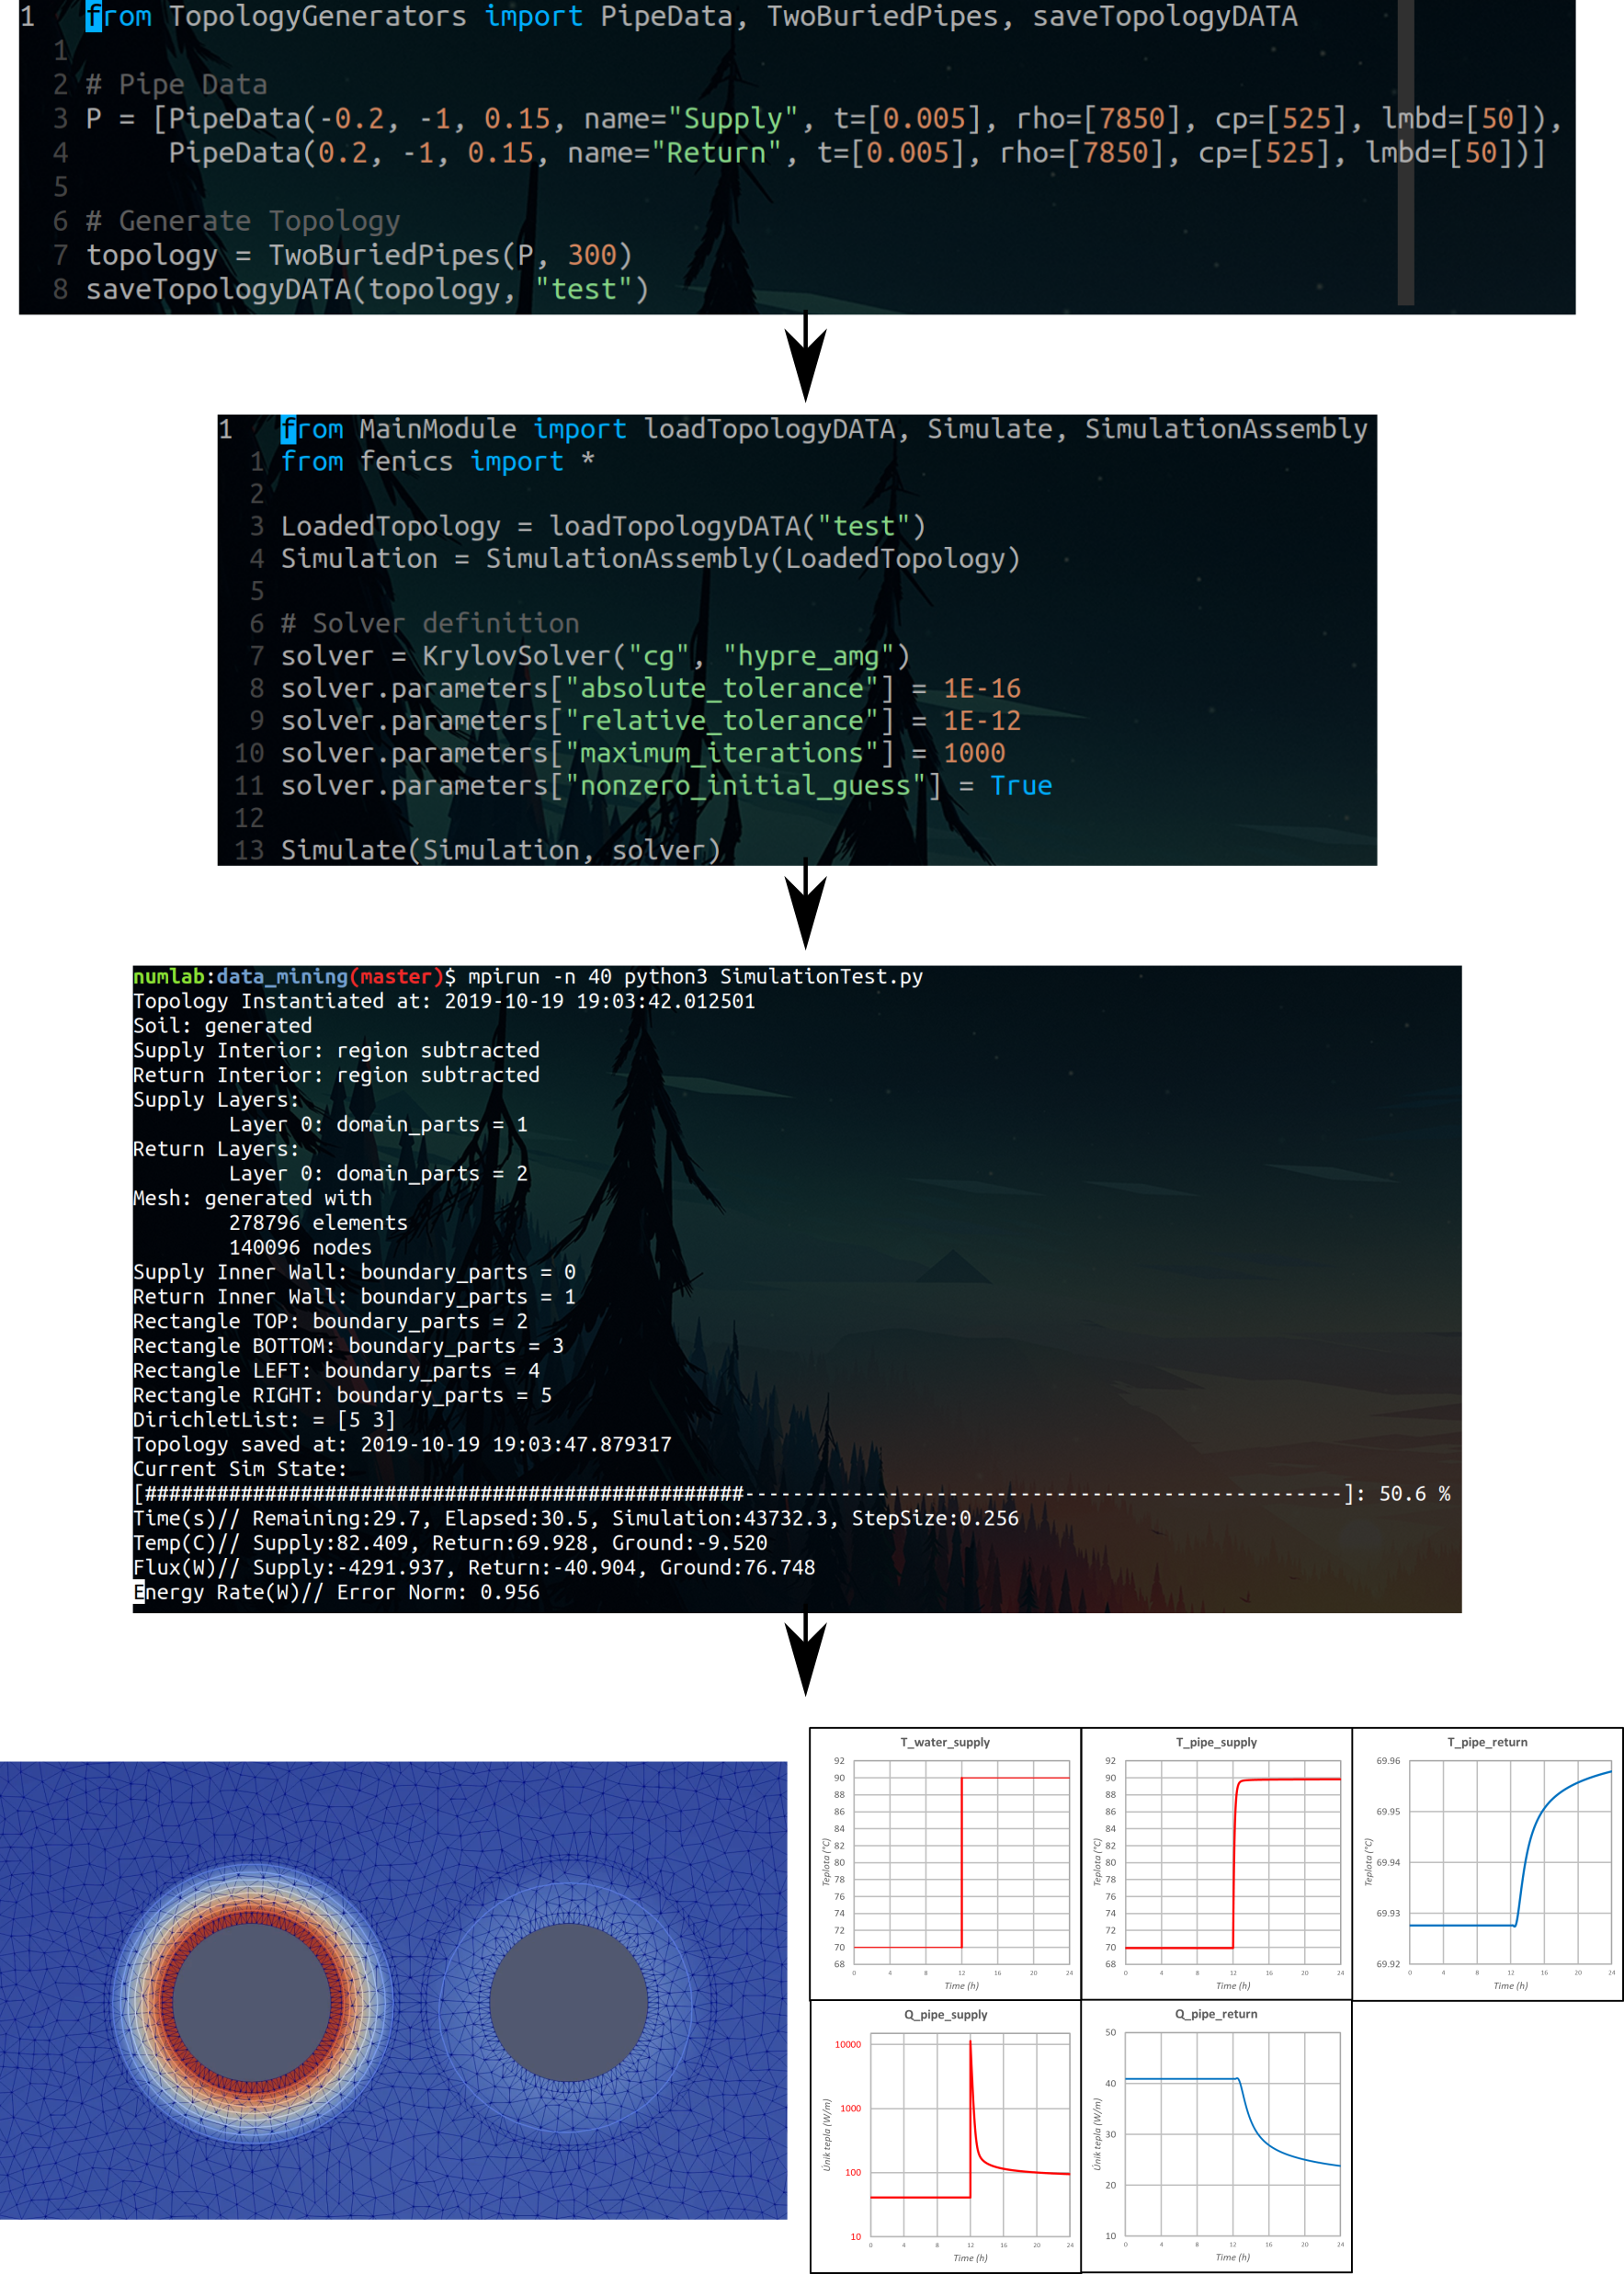
\includegraphics[scale=0.65]{figures/fenics_sim_pipes}
\end{center}
\caption{Nástroj pro simulaci radiálního šíření tepla}
\label{fig:}
\end{figure}
\subsection{Optimalizační nástroj LOFI}
Nástroj LOFI je také ve stavu funkčního prototypu. Plánovač úloh, API pro OMC,
tři funkční optimalizační algoritmy (hejnový algoritmus PSO, hejnový algoritmus
s náhodnou adaptací GRAPSO a evoluční strategie s adaptací vzorkovacího
prostoru OPLES), vizualizační callback a interaktivní konzole jsou otestovány.
Samotný nástroj LOFI je publikován v konferenčním sborníku
\textit{SDEWES Cologne 2020}. LOFI bylo otestováno pro optimalizaci/nalezení
advektivního schématu, řízení okrajové podmínky pro problém vedení tepla a
učení neuronové síťě pro zachycení testovacího modelu Lotka-Voltera. Všechny
tři modely byly implementovány v jazyce modelica a kompilovány pomocí OMC. 
\begin{figure}[h]
\begin{center}
  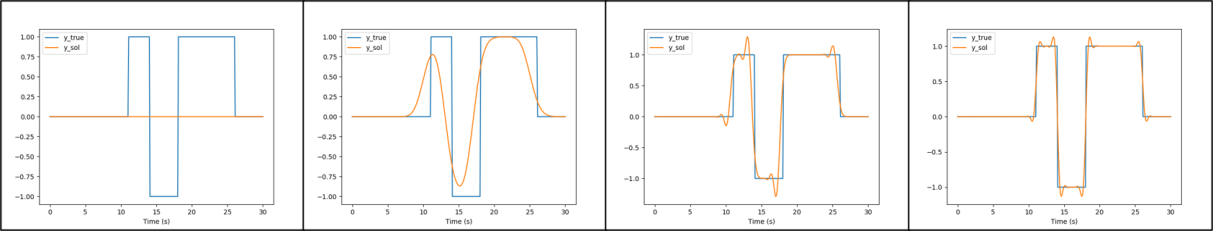
\includegraphics[width=\textwidth]{figures/Advection_GRAPSO}
\end{center}
\caption{Průběh optimalizace advektivního schématu algoritmem GRAPSO}
\label{fig:Advection_GRAPSO}
\end{figure}
\begin{figure}[h]
\begin{center}
  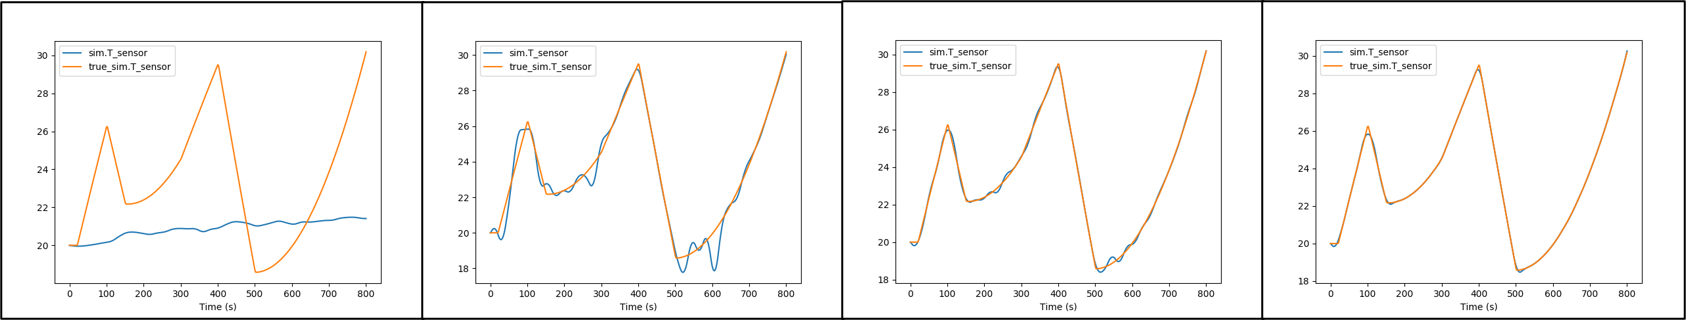
\includegraphics[width=\textwidth]{figures/Inverse_OPLES}
\end{center}
\caption{Průběh optimalizace okrajové podmínky v problému vedení tepla
algoritmem OPLES}
\label{fig:Advection_GRAPSO}
\end{figure}
\begin{figure}[h]
\begin{center}
  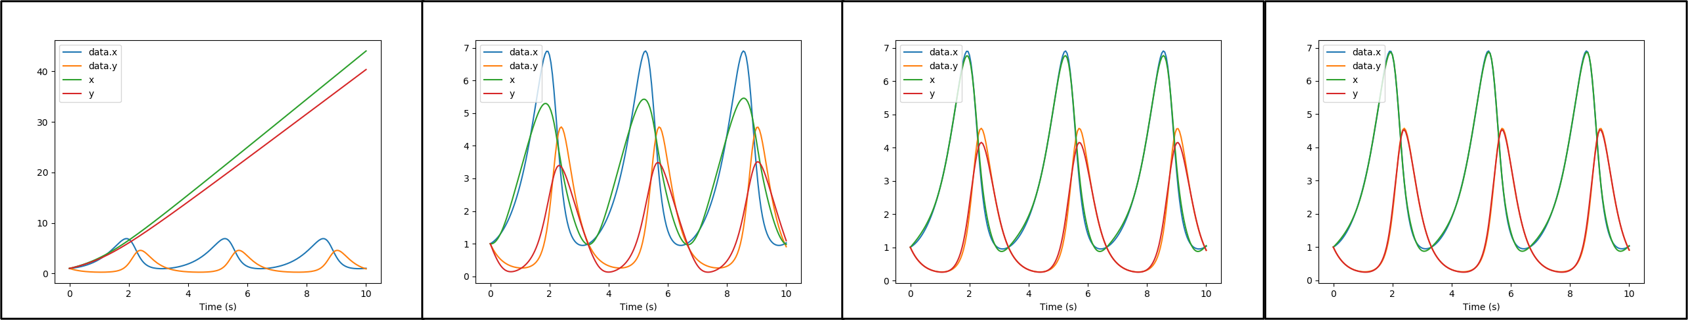
\includegraphics[width=\textwidth]{figures/LotkaVoltera_NN_OPLES}
\end{center}
\caption{Průběh optimalizace neuronové sítě s 50 neurony ve vnitřní vrstvě
reprezentující ODR systém Lotka-Voltera, kde optimalizace proběhla pomocí algoritmu OPLES}
\label{fig:Advection_GRAPSO}
\end{figure}

